\addtocontents{toc}{\protect\setlength{\cftsecnumwidth}{13mm}}


\chapter{Diseño}
A continuación, se describe cada caso de uso del PFG siguiendo el orden establecido en el Mapeo de Requerimientos – Casos de Uso. Posteriormente, para agregar valor a la documentación del software, se incluye un diagrama de despliegue, un diagrama de paquetes y un diagrama de estados.  
\section{Gestionar Lugar}

\begin{table}[H]
    \begin{tabular}{@{} *5l @{}} \toprule
    \textbf{Caso de Uso} & Gestionar Lugar \\ \midrule
    Actor & Gerente \\ 
    Descripción & El gerente gestiona un lugar. \\ 
    Propósito & El gerente quiere gestionar un lugar. \\ \midrule
    Precondiciones & El gerente inicia su navegador web. \\ \midrule
    Postcondiciones & Existe un lugar. \\ \midrule
    \multirow{4}{*}{Curso Básico}
        & \parbox{0.75\linewidth}{ 
                1. El gerente visita la página de Lugares. \\
                2. El gerente hace click en el botón Nuevo. \\
                3. El sistema muestra la página del formulario de lugar. \\
                4. El gerente ingresa la información correspondiente y envía los datos haciendo click en el botón Guardar. \\
                5. El sistema registra el lugar.  \\
                6. El sistema muestra la página de Lugares.   
        } \\ \midrule
        \multirow{2}{*}{Excepciones}
        & \parbox{0.75\linewidth}{ 
            1. El sistema no puede registrar el lugar dada una falla en la base de datos. \\
            2. El gerente puede salir de la página del formulario de lugar en cualquier momento antes de eliminar haciendo click en Cancelar.
        }  \\  \bottomrule
     \hline
    \end{tabular}
        \caption{Gestionar Lugar - Caso de Uso (1)}
        \label{tab:tabcu-lugar}
\end{table}


\begin{table}[H]
    \begin{tabular}{@{} *5l @{}} \toprule
    \textbf{Caso de Uso} & Gestionar Lugar \\ \midrule
    Actor & Gerente \\ 
    Descripción & El gerente gestiona un lugar. \\ 
    Propósito & El gerente quiere gestionar un lugar. \\ \midrule
    Precondiciones & El gerente inicia su navegador web. Existe el lugar. \\ \midrule
    Postcondiciones & Existe un lugar con nuevos datos. \\ \midrule
    \multirow{4}{*}{Curso Básico}
        & \parbox{0.75\linewidth}{ 
                1. El gerente visita la página de Lugares. \\
                2. El gerente hace click en el botón Modificar de un lugar. \\
                3. El sistema muestra la página del formulario de lugar. \\
                    3.1 El sistema recuperara datos del lugar para intentar poblar el formulario. \\
                4. El gerente ingresa la información correspondiente y envía los datos haciendo click en el botón Guardar. \\
                5. El sistema actualiza el lugar.  \\
                6. El sistema muestra la página de Lugares.   
        } \\ \midrule
        \multirow{2}{*}{Excepciones}
        & \parbox{0.75\linewidth}{ 
            1. El sistema no puede actualizar el lugar dada una falla en la base de datos. \\
            2. El gerente puede salir de la página del formulario de lugar en cualquier momento antes de eliminar haciendo click en Cancelar.
        }  \\  \bottomrule
     \hline
    \end{tabular}
        \caption{Gestionar Lugar - Caso de Uso (2)}
        \label{tab:tabcu-lugar2}
\end{table}


\begin{table}[H]
    \begin{tabular}{@{} *5l @{}} \toprule
    \textbf{Caso de Uso} & Gestionar Lugar \\ \midrule
    Actor & Gerente \\ 
    Descripción & El gerente gestiona un lugar. \\ 
    Propósito & El gerente quiere gestionar un lugar. \\ \midrule
    Precondiciones & El gerente inicia su navegador web. Existe el lugar.\\ \midrule
    Postcondiciones & Se eliminó un lugar. \\ \midrule
    \multirow{4}{*}{Curso Básico}
        & \parbox{0.75\linewidth}{ 
                1. El gerente visita la página de Lugares. \\
                2. El gerente hace click en el botón Detalles de un Lugar. \\
                3. El sistema muestra la página de Detalles de un Lugar. \\
                    3.1 El sistema recupera datos del Lugar para mostrar los detalles. \\
                4. El gerente elimina el lugar haciendo click en el botón Eliminar. \\
                5. El sistema elimina el lugar.  \\
                6. El sistema muestra la página de Lugares.   
        } \\ \midrule
        \multirow{2}{*}{Excepciones}
        & \parbox{0.75\linewidth}{ 
            1. El sistema no puede eliminar el lugar dada una falla en la base de datos. \\
            2. El gerente puede salir de la página de detalles en cualquier momento antes de eliminar haciendo click en Cancelar.
        }  \\  \bottomrule
     \hline
    \end{tabular}
        \caption{Gestionar Lugar - Caso de Uso (3)}
        \label{tab:tabcu-lugar3}
\end{table}
    
    
    \begin{figure}[H]
        \centering
        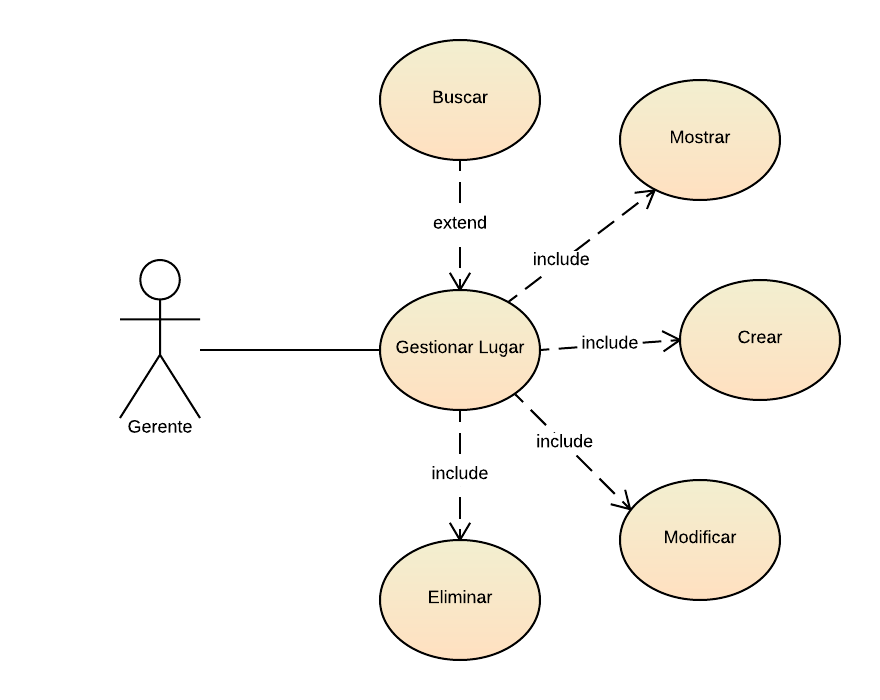
\includegraphics[width=0.85\textwidth]{chapter10/lugar-uc}
        \caption{Gestionar Lugar - Diagrama de Caso de Uso}
        \label{fig:lugar-uc}
    \end{figure}
    
    \begin{figure}[H]
        \centering
        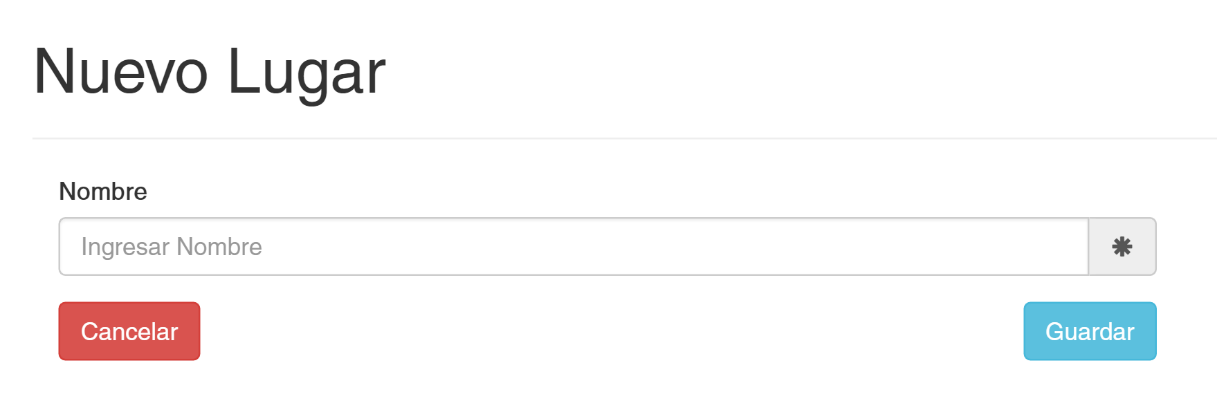
\includegraphics[width=1\textwidth]{chapter10/lugar-int}
        \caption{Gestionar Lugar - Interfaz Tentativa }
        \label{fig:lugar-int}
    \end{figure}
    
    \begin{figure}[H]
        \centering
        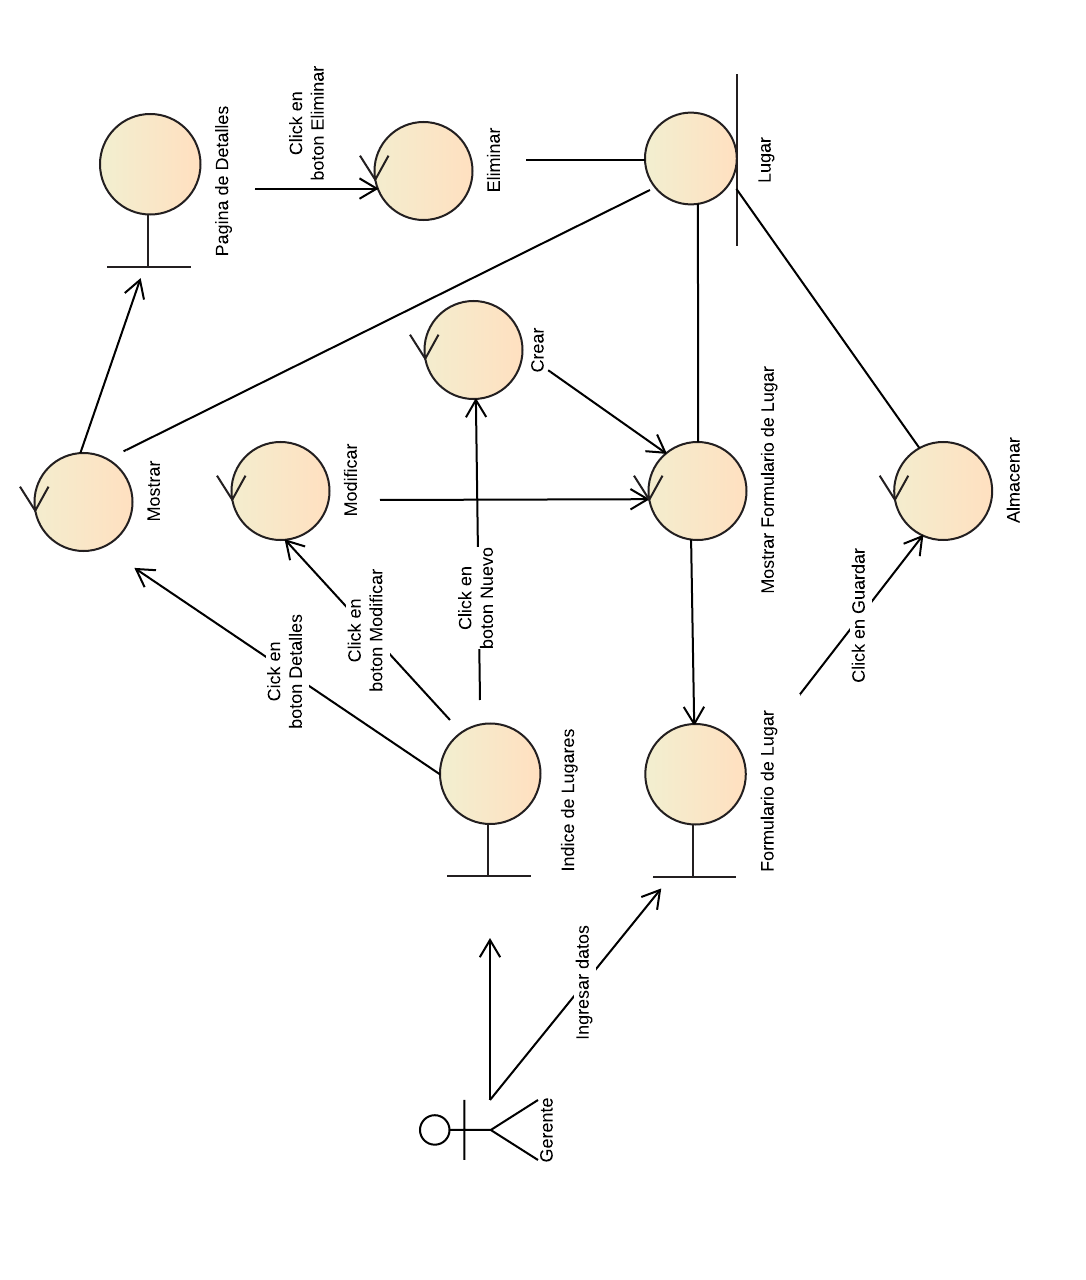
\includegraphics[width=1\textwidth]{chapter10/lugar-rob}
        \caption{Gestionar Lugar - Diagrama de Robustez}
        \label{fig:lugar-rob}
    \end{figure}
    
    \begin{figure}[H]
        \centering
        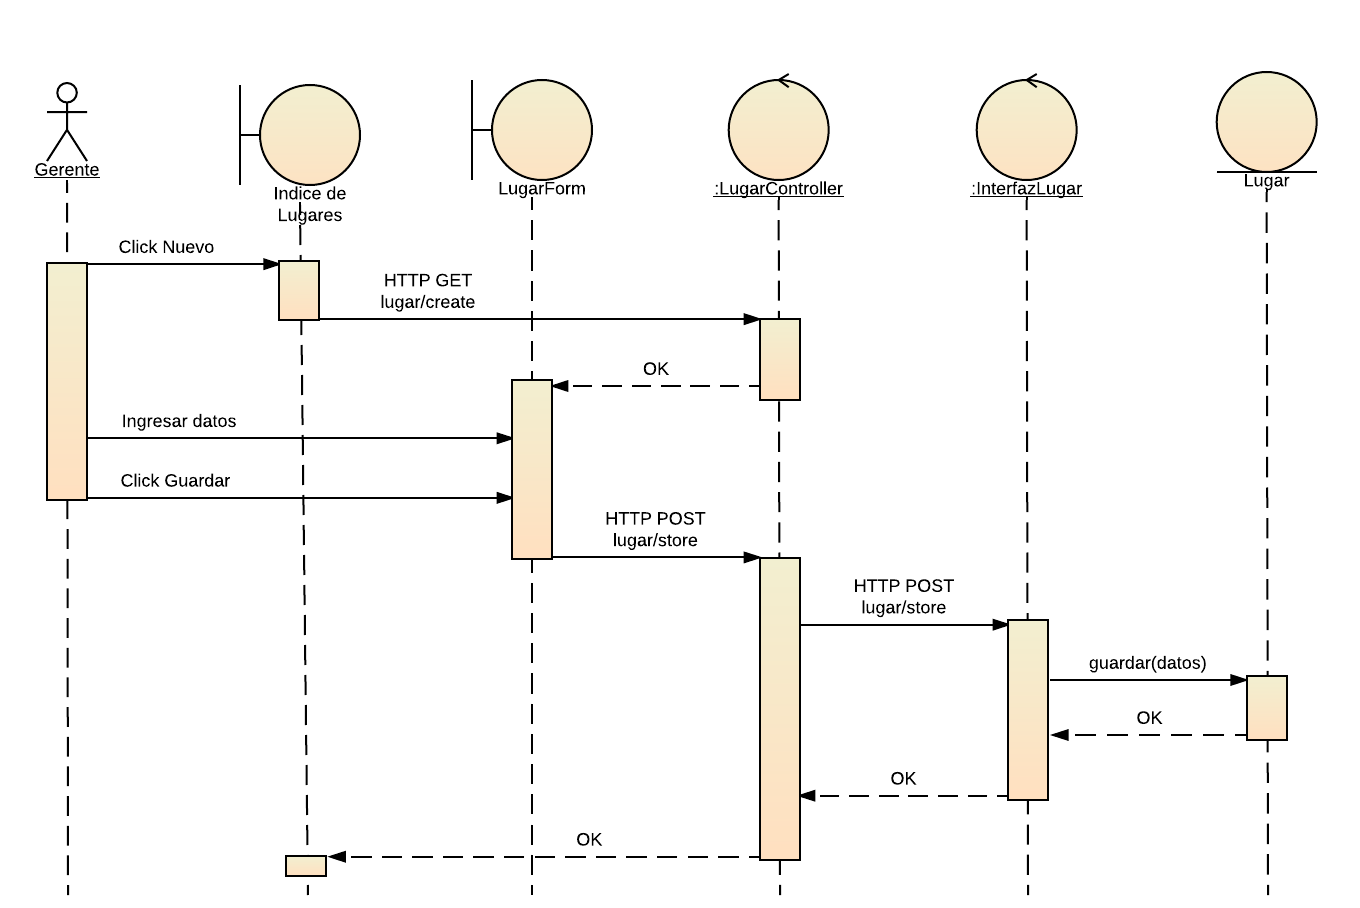
\includegraphics[width=.8\textwidth]{chapter10/lugar-seq-create}
        \caption{Gestionar Lugar - Diagrama de Secuencia (1) }
        \label{fig:lugar-seq-create}
    \end{figure}
    
    \begin{figure}[H]
        \centering
        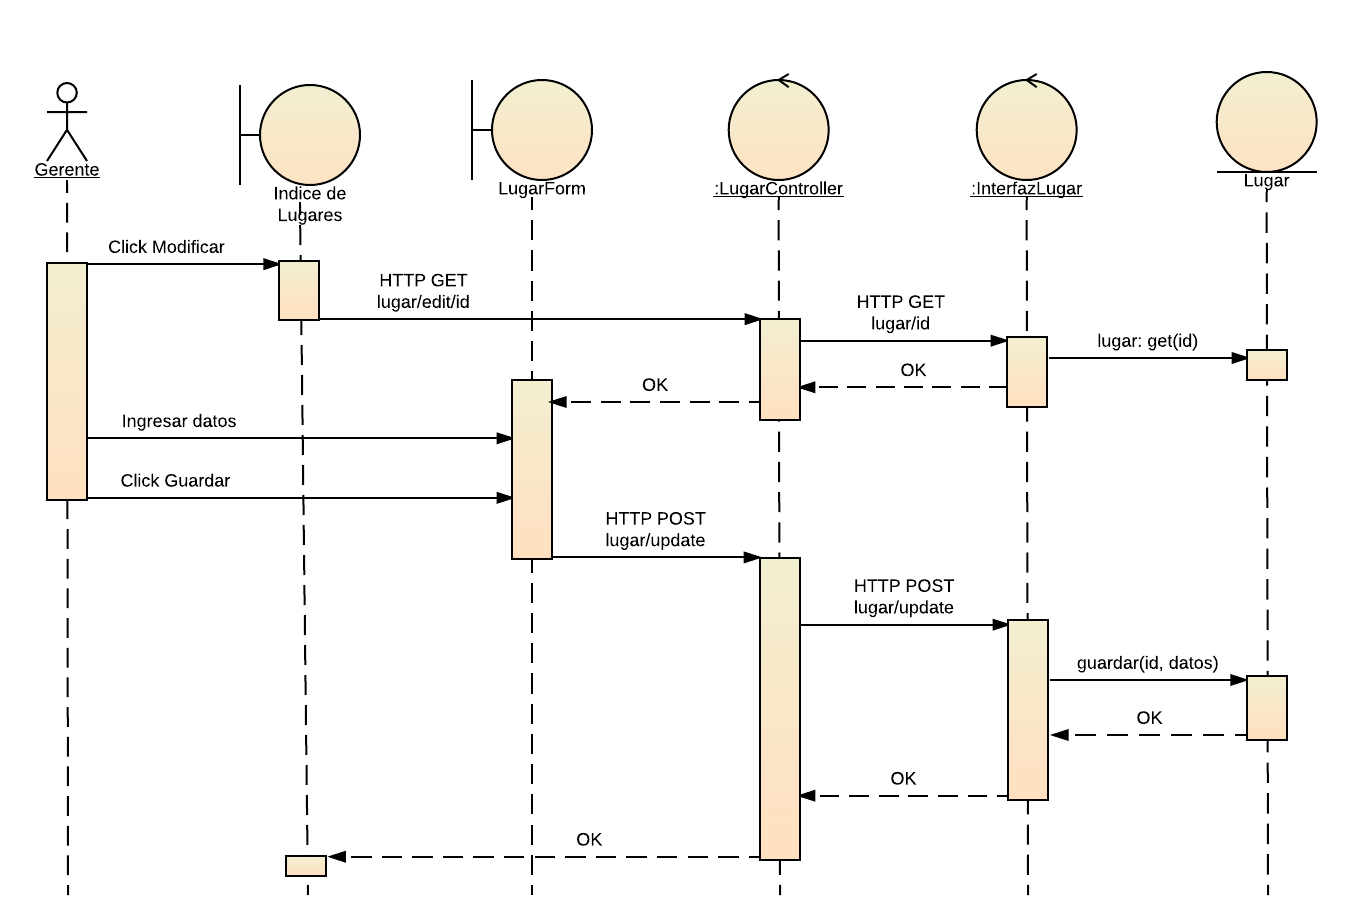
\includegraphics[width=.8\textwidth]{chapter10/lugar-seq-edit}
        \caption{Gestionar Lugar - Diagrama de Secuencia (2) }
        \label{fig:lugar-seq-edit}
    \end{figure}
    
    \begin{figure}[H]
        \centering
        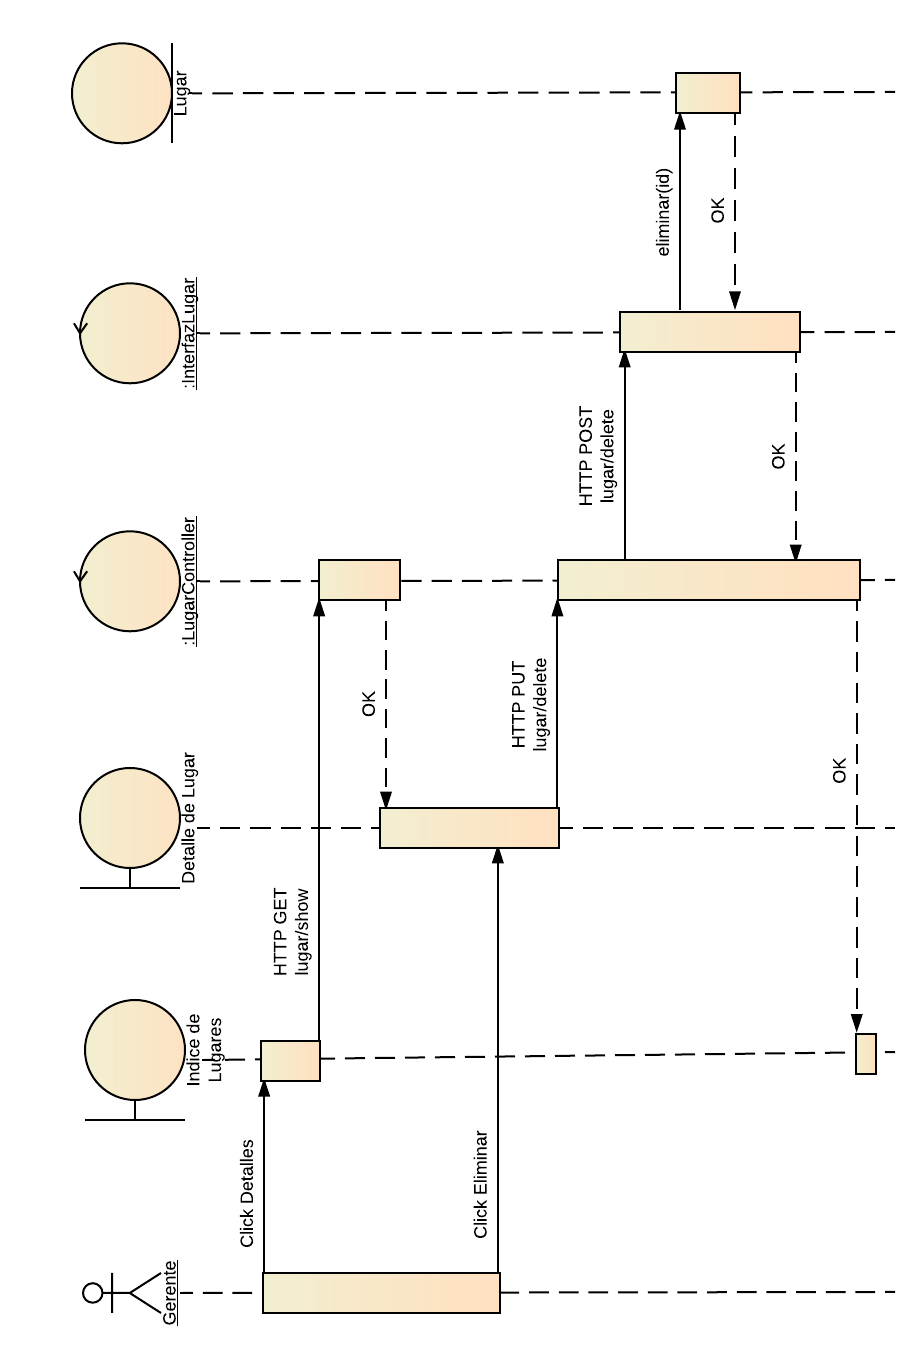
\includegraphics[width=.8\textwidth]{chapter10/lugar-seq-del}
        \caption{Gestionar Lugar - Diagrama de Secuencia (3) }
        \label{fig:lugar-seq-del}
    \end{figure}

\section{Gestionar Cámara}

\begin{table}[H]
    \begin{tabular}{@{} *5l @{}} \toprule
    \textbf{Caso de Uso} & Gestionar Cámara \\ \midrule
    Actor & Gerente \\ 
    Descripción & El gerente gestiona una cámara. \\ 
    Propósito & El gerente quiere gestionar una cámara. \\ \midrule
    Precondiciones & El gerente inicia su navegador web. \\ \midrule
    Postcondiciones & Existe una cámara. \\ \midrule
    \multirow{4}{*}{Curso Básico}
        & \parbox{0.75\linewidth}{ 
                1. El gerente visita la página de Cámaras. \\
                2. El gerente hace click en el botón Nuevo. \\
                3. El sistema muestra la página del Formulario de Cámara. \\
                4. El gerente ingresa la información correspondiente y envía los datos haciendo click en el botón Guardar. \\
                5. El sistema registra la Cámara.  \\
                6. El sistema muestra la página de Cámaras.   
        } \\ \midrule
        \multirow{2}{*}{Excepciones}
        & \parbox{0.75\linewidth}{ 
            1. El sistema no puede registrar la cámara dada una falla en la base de datos. \\
            2. El gerente puede salir de la página del Formulario de Cámara en cualquier momento antes de eliminar haciendo click en Cancelar.
        }  \\  \bottomrule
     \hline
    \end{tabular}
        \caption{Gestionar Lugar - Caso de Uso (1)}
        \label{tab:tabcu-cam}
\end{table}


\begin{table}[H]
    \begin{tabular}{@{} *5l @{}} \toprule
    \textbf{Caso de Uso} & Gestionar Cámara \\ \midrule
    Actor & Gerente \\ 
    Descripción & El gerente gestiona una Cámara. \\ 
    Propósito & El gerente quiere gestionar una Cámara. \\ \midrule
    Precondiciones & El gerente inicia su navegador web. \\ Existe un lugar. \\ Existe la Cámara. \\ \midrule
    Postcondiciones & Existe una Cámara con nuevos datos. \\ \midrule
    \multirow{4}{*}{Curso Básico}
        & \parbox{0.75\linewidth}{ 
                1. El gerente visita la página de Cámara. \\
                2. El gerente hace click en el botón Modificar de una Cámara. \\
                3. El sistema muestra la página del Formulario de Cámara. \\
                    3.1 El sistema recuperara datos de la Cámara para intentar poblar el formulario. \\
                4. El gerente ingresa la información correspondiente y envía los datos haciendo click en el botón Guardar. \\
                5. El sistema actualiza la Cámara.  \\
                6. El sistema muestra la página de Cámaras.   
        } \\ \midrule
        \multirow{2}{*}{Excepciones}
        & \parbox{0.75\linewidth}{ 
            1. El sistema no puede actualizar la Cámara dada una falla en la base de datos. \\
            2. El gerente puede salir de la página del formulario de Cámara en cualquier momento antes de eliminar haciendo click en Cancelar.
        }  \\  \bottomrule
     \hline
    \end{tabular}
        \caption{Gestionar Lugar - Caso de Uso (2)}
        \label{tab:tabcu-cam2}
\end{table}


\begin{table}[H]
    \begin{tabular}{@{} *5l @{}} \toprule
    \textbf{Caso de Uso} & Gestionar Cámara \\ \midrule
    Actor & Gerente \\ 
    Descripción & El gerente gestiona una Cámara. \\ 
    Propósito & El gerente quiere gestionar una Cámara. \\ \midrule
    Precondiciones & El gerente inicia su navegador web. Existe un lugar. Existe la Cámara.\\ \midrule
    Postcondiciones & Se eliminó una Cámara. \\ \midrule
    \multirow{4}{*}{Curso Básico}
        & \parbox{0.75\linewidth}{ 
                1. El gerente visita la página de Cámaras. \\
                2. El gerente hace click en el botón Detalles de una Cámara. \\
                3. El sistema muestra la página de Detalles de una Cámara. \\
                    3.1 El sistema recupera datos de  la Cámara para mostrar los detalles. \\
                4. El gerente elimina la Cámara haciendo click en el botón Eliminar. \\
                5. El sistema elimina la Cámara.  \\
                6. El sistema muestra la página de Cámaras.   
        } \\ \midrule
        \multirow{2}{*}{Excepciones}
        & \parbox{0.75\linewidth}{ 
            1. El sistema no puede eliminar la Cámara dada una falla en la base de datos. \\
            2. El gerente puede salir de la página de detalles en cualquier momento antes de eliminar haciendo click en Cancelar.
        }  \\  \bottomrule
     \hline
    \end{tabular}
        \caption{Gestionar Lugar - Caso de Uso (3)}
        \label{tab:tabcu-cam3}
\end{table}
    
    
    \begin{figure}[H]
        \centering
        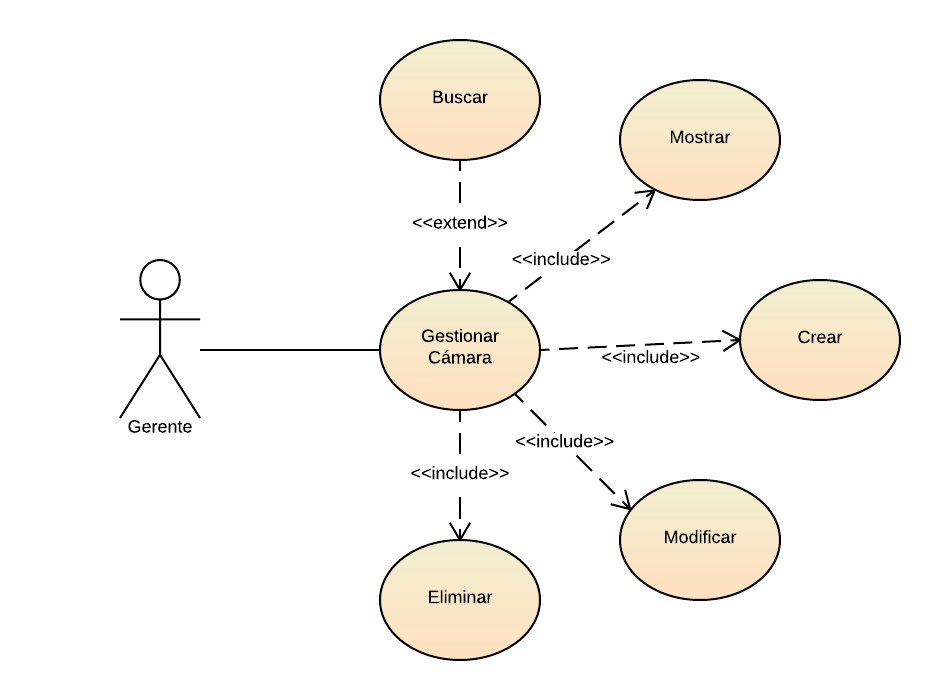
\includegraphics[width=0.85\textwidth]{chapter10/uc-cam}
        \caption{Gestionar Lugar - Diagrama de Caso de Uso}
        \label{fig:uc-cam}
    \end{figure}
    
    % \begin{figure}[H]
    %     \centering
    %     \includegraphics[width=1\textwidth]{chapter10/camara-int}
    %     \caption{Gestionar Lugar - Interfaz Tentativa }
    %     \label{fig:lugar-int}
    % \end{figure}
      \begin{landscape}
    \begin{figure}[H]
        \centering
        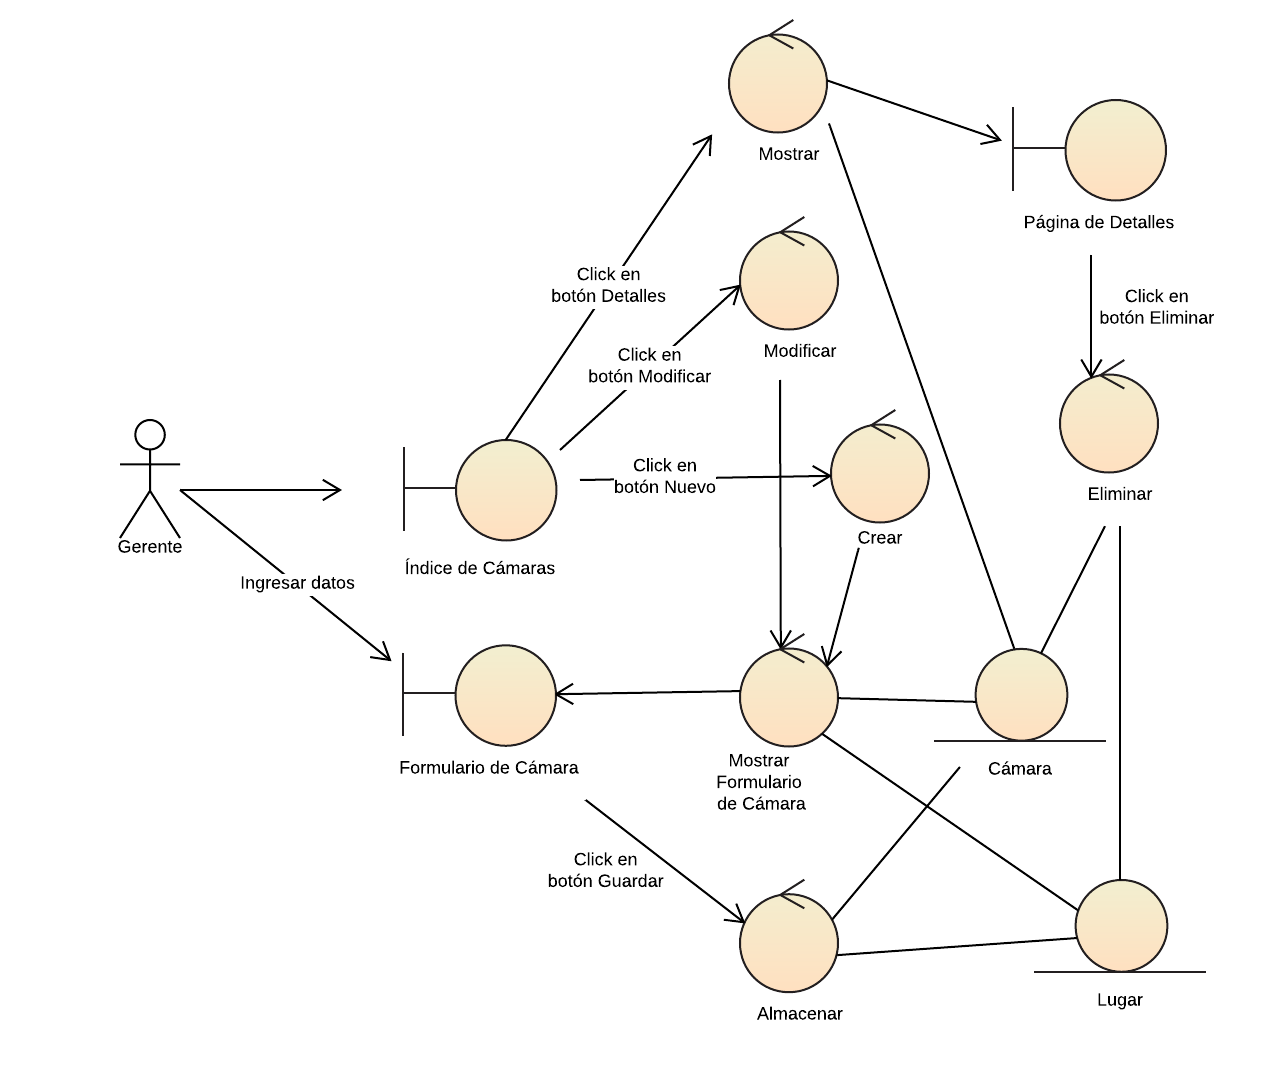
\includegraphics[width=1\textwidth]{chapter10/rob-cam}
        \caption{Gestionar Cámara - Diagrama de Robustez}
        \label{fig:rob-cam}
    \end{figure}
  
    \begin{figure}[H]
        \centering
        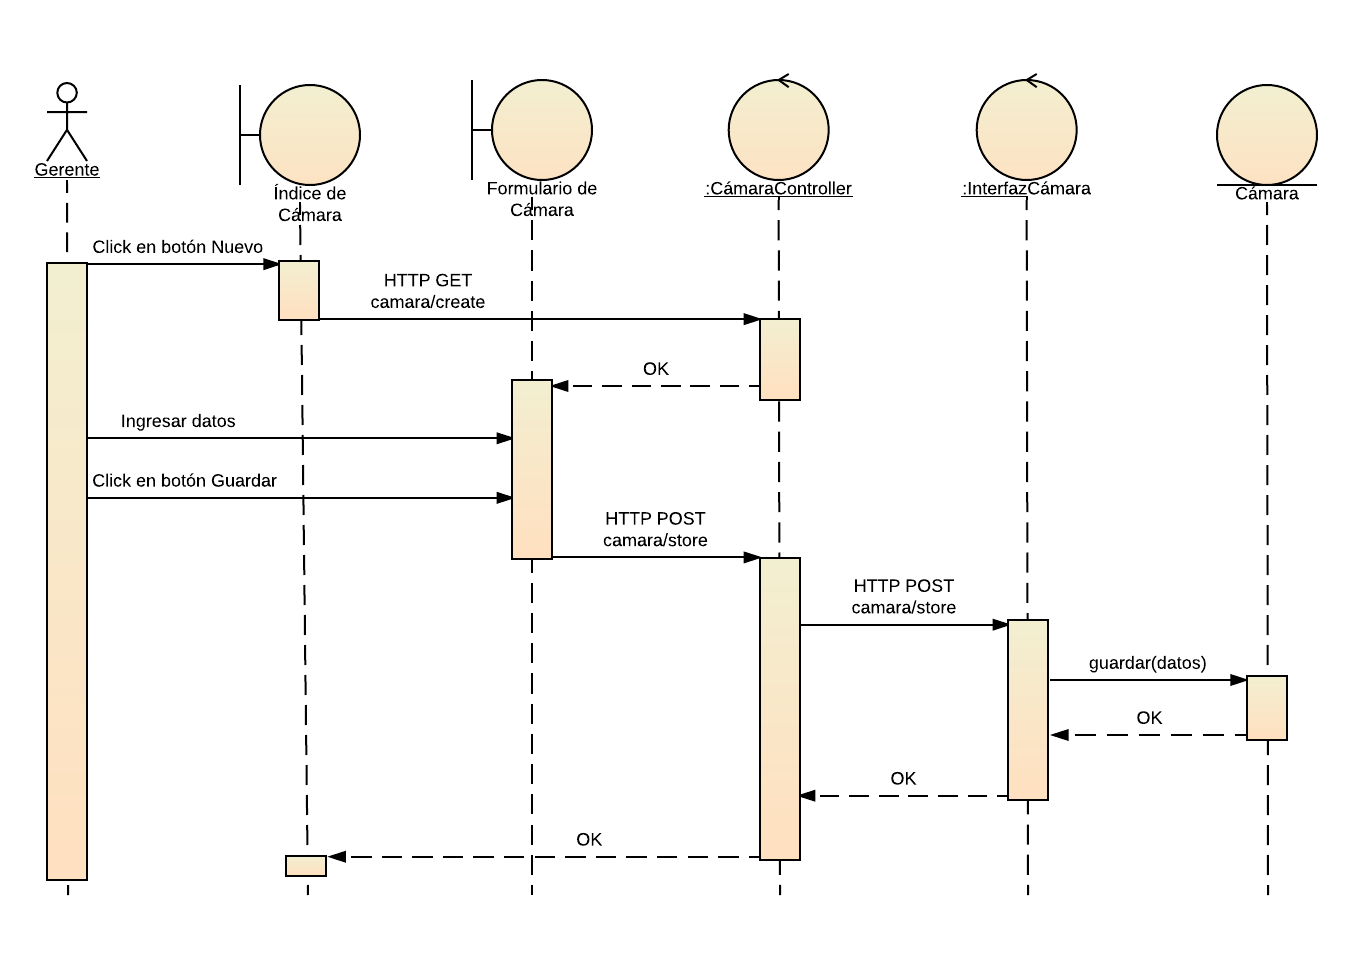
\includegraphics[width=1.1\textwidth]{chapter10/seq-cam-nu}
        \caption{Gestionar Cámara - Diagrama de Secuencia (1) }
        \label{fig:seq-cam-nu}
    \end{figure}
    
    \begin{figure}[H]
        \centering
        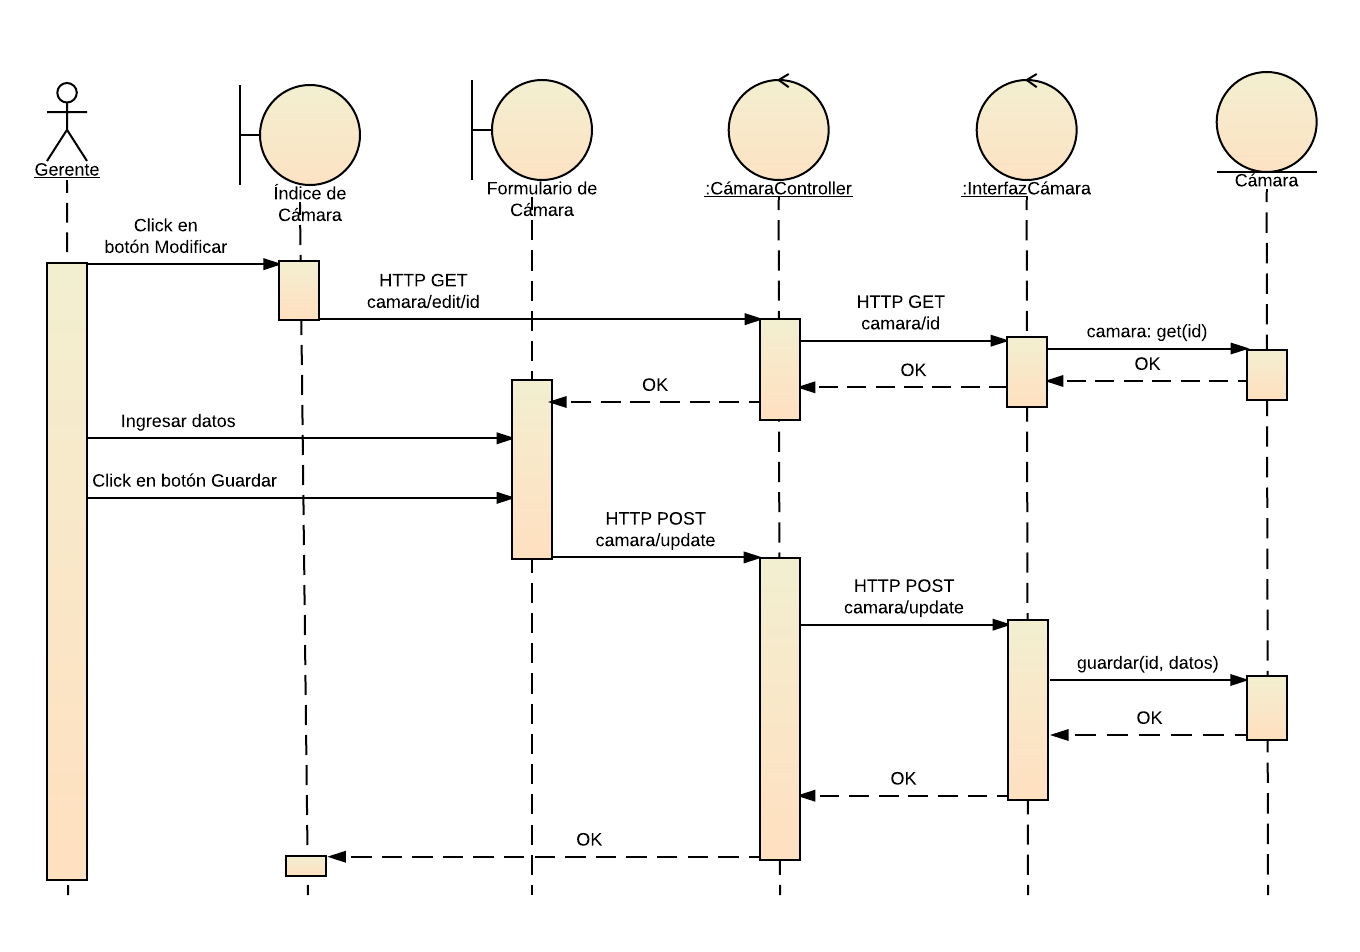
\includegraphics[width=1.1\textwidth]{chapter10/seq-cam-mo}
        \caption{Gestionar Cámara - Diagrama de Secuencia (2) }
        \label{fig:seq-cam-mo}
    \end{figure}
    
    \begin{figure}[H]
        \centering
        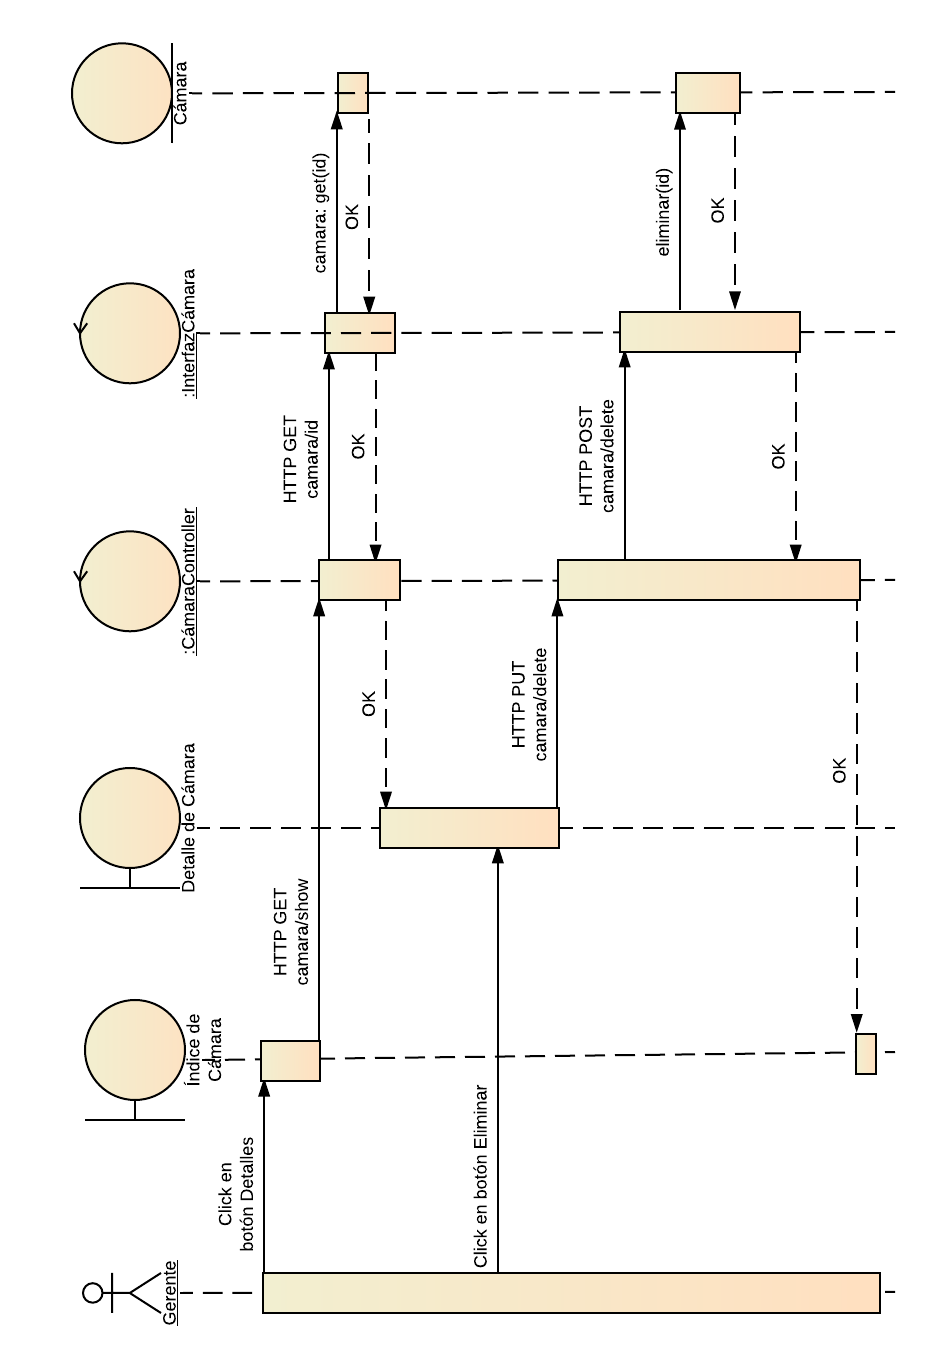
\includegraphics[width=1.1\textwidth]{chapter10/seq-cam-el}
        \caption{Gestionar Cámara - Diagrama de Secuencia (3) }
        \label{fig:seq-cam-el}
    \end{figure}
    \end{landscape}

\section{Gestionar Matrícula}

\begin{longtable}{@{} p{3cm} p{10cm} @{}} \toprule
    \textbf{Caso de Uso}    & Gestionar Matrícula \\ \midrule
    Actor                   & Gerente \\ \cmidrule{1-2}
    Descripción             & El gerente gestiona una Matrícula. \\ \cmidrule{1-2}
    Propósito               & El gerente quiere gestionar una Matrícula. \\ \cmidrule{1-2}
    Precondiciones          & El gerente inicia su navegador web. Existe el Propietario. Existe la Matrícula. \\ \cmidrule{1-2} 
    Postcondiciones         & Existe una nueva Matrícula. \\ \cmidrule{1-2} 
                            & 1. El gerente visita la página de Propietarios. \\ 
                            & 2. El gerente hace click en el botón Detalles de un Propietario. \\
                            & 2.1 El sistema recupera los datos del Propietario para mostrar la pagina de detalles. \\
    Curso Básico            & 3. El gerente hace click en el boton Nuevo. \\
                            & 4. El sistema muestra la página del Formulario de Matrícula. \\
                            & 5. El gerente ingresa la información correspondiente y envía los datos haciendo click en el botón Guardar. \\ 
                            & 6. El sistema registra la Matrícula. \\ 
                            & 7. El sistema muestra la página de Detalles del Propietario con la nueva Matrícula. \\ \cmidrule{1-2}
    Excepciones             & 1. El sistema no puede registrar la Matrícula dada una falla en la base de datos. \\
                            & 2. El gerente puede salir de la página del formulario de Matrícula en cualquier momento antes de eliminar haciendo click en Cancelar. \\ \bottomrule
   \caption{Gestionar Matrícula - Caso de Uso (3)} \label{tab:tabcu-matri1} \\
   \end{longtable}

\begin{longtable}{@{} p{3cm} p{10cm} @{}} \toprule
    \textbf{Caso de Uso}    & Gestionar Matrícula \\ \midrule
    Actor                   & Gerente \\ \cmidrule{1-2}
    Descripción             & El gerente gestiona una Matrícula. \\ \cmidrule{1-2}
    Propósito               & El gerente quiere gestionar una Matrícula. \\ \cmidrule{1-2}
    Precondiciones          & El gerente inicia su navegador web. Existe el Propietario. Existe la Matrícula. \\ \cmidrule{1-2} 
    Postcondiciones         & Existe una Matrícula con nuevos datos. \\ \cmidrule{1-2} 
                            & 1. El gerente visita la página de Propietarios. \\ 
                            & 2. El gerente hace click en el botón Detalles de un Propietario. \\
                            & 2.1 El sistema recupera los datos del Propietario para mostrar la pagina de detalles. \\
    Curso Básico            & 3. El gerente hace click en el boton Modificar de una Matrícula. \\
                            & 4. El sistema muestra la página del Formulario de Matrícula. \\
                            & 4.1. El sistema recupera datos de la Matrícula para intentar poblar el formulario. \\
                            & 6. El gerente ingresa la información correspondiente y envía los datos haciendo click en el botón Guardar. \\ 
                            & 7. El sistema actualiza la Matrícula. \\ 
                            & 8. El sistema muestra la página de Detalles del Propietario con la nueva Matrícula. \\ \cmidrule{1-2}
    Excepciones             & 1. El sistema no puede actualizar la Matrícula dada una falla en la base de datos. \\
                            & 2. El gerente puede salir de la página del formulario de Matrícula en cualquier momento antes de eliminar haciendo click en Cancelar. \\ \bottomrule
   \caption{Gestionar Matrícula - Caso de Uso (3)} \label{tab:tabcu-matri2} \\
   \end{longtable}

 \begin{longtable}{@{} p{3cm} p{10cm} @{}} \toprule
    \textbf{Caso de Uso}    & Gestionar Matrícula \\ \midrule
    Actor                   & Gerente \\ \cmidrule{1-2}
    Descripción             & El gerente gestiona una Matrícula. \\ \cmidrule{1-2}
    Propósito               & El gerente quiere gestionar una Matrícula. \\ \cmidrule{1-2}
    Precondiciones          & El gerente inicia su navegador web. Existe el Propietario. Existe la Matrícula. \\ \cmidrule{1-2} 
    Postcondiciones         & Se eliminó una Matrícula. \\ \cmidrule{1-2} 
                            & 1. El gerente visita la página de Propietarios. \\ 
                            & 2. El gerente hace click en el botón Detalles de un Propietario. \\
                            & 2.1 El sistema recupera los datos del Propietario para mostrar la pagina de detalles. \\
    Curso Básico            & 3. El gerente selecciona una Matrícula haciendo click en ell boton Detalles. \\
                            & 4. El sistema muestra la página de Detalles de una Matrícula. \\
                            & 5. El gerente elimina la Matrícula haciendo click en el botón Eliminar. \\
                            & 6. El sistema elimina la Matrícula. \\ \cmidrule{1-2}
    Excepciones             & 1. El sistema no puede eliminar la Matrícula dada una falla en la base de datos. \\
                            & 2. El gerente puede salir de la página de detalles en cualquier momento antes de eliminar haciendo click en Cancelar. \\ \bottomrule
   \caption{Gestionar Matrícula - Caso de Uso (3)} \label{tab:tabcu-matri3} \\
   \end{longtable}
  
 
    \begin{figure}[H]
        \centering
        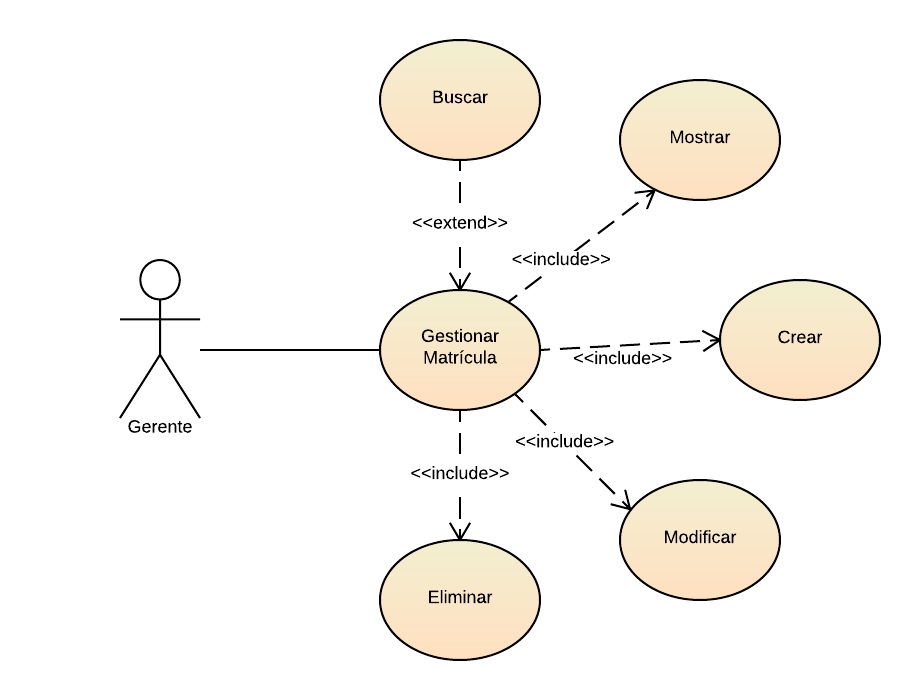
\includegraphics[width=0.8\textwidth]{chapter10/uc-matri}
        \caption{Gestionar Matrícula - Diagrama de Caso de Uso}
        \label{fig:uc-matri}
    \end{figure}
    
    % \begin{figure}[H]
    %     \centering
    %     \includegraphics[width=1\textwidth]{chapter10/camara-int}
    %     \caption{Gestionar Lugar - Interfaz Tentativa }
    %     \label{fig:lugar-int}
    % \end{figure}
\begin{landscape}
    \begin{figure}[H]
        \centering
        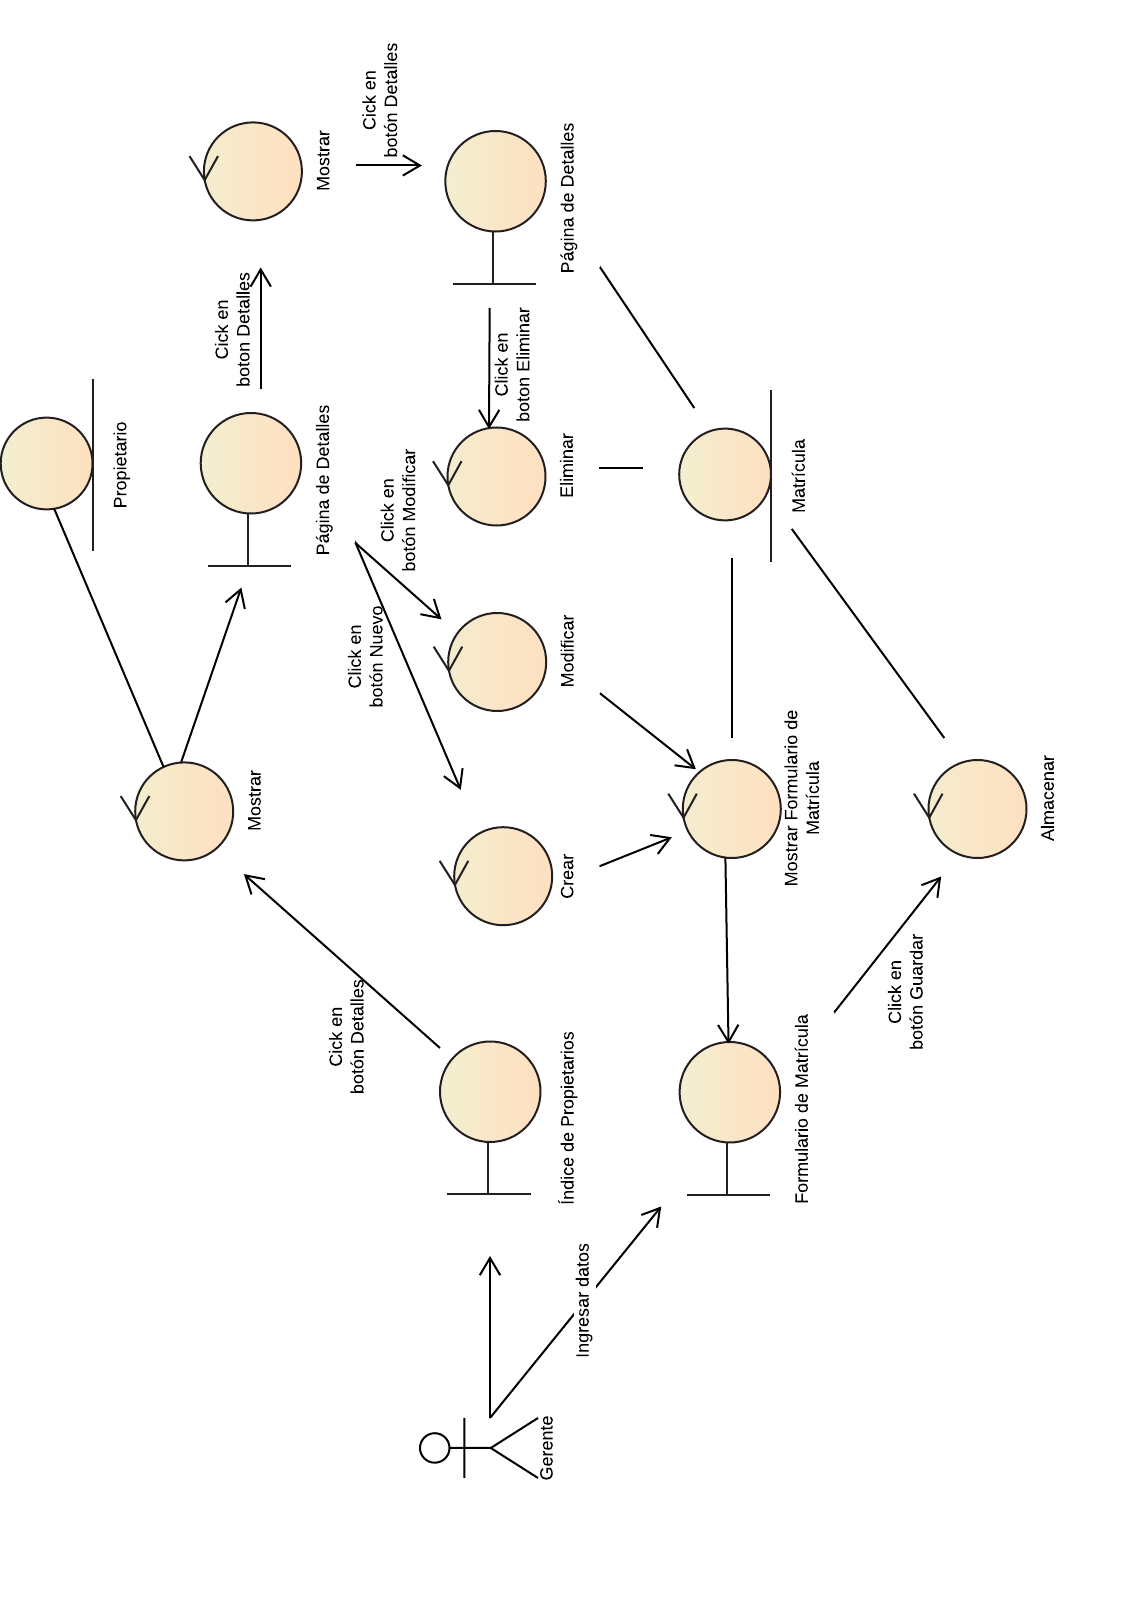
\includegraphics[width=1.1\textwidth]{chapter10/rob-matri}
        \caption{Gestionar Matrícula - Diagrama de Robustez}
        \label{fig:rob-matri}
    \end{figure}
    \begin{figure}[H]
        \centering
        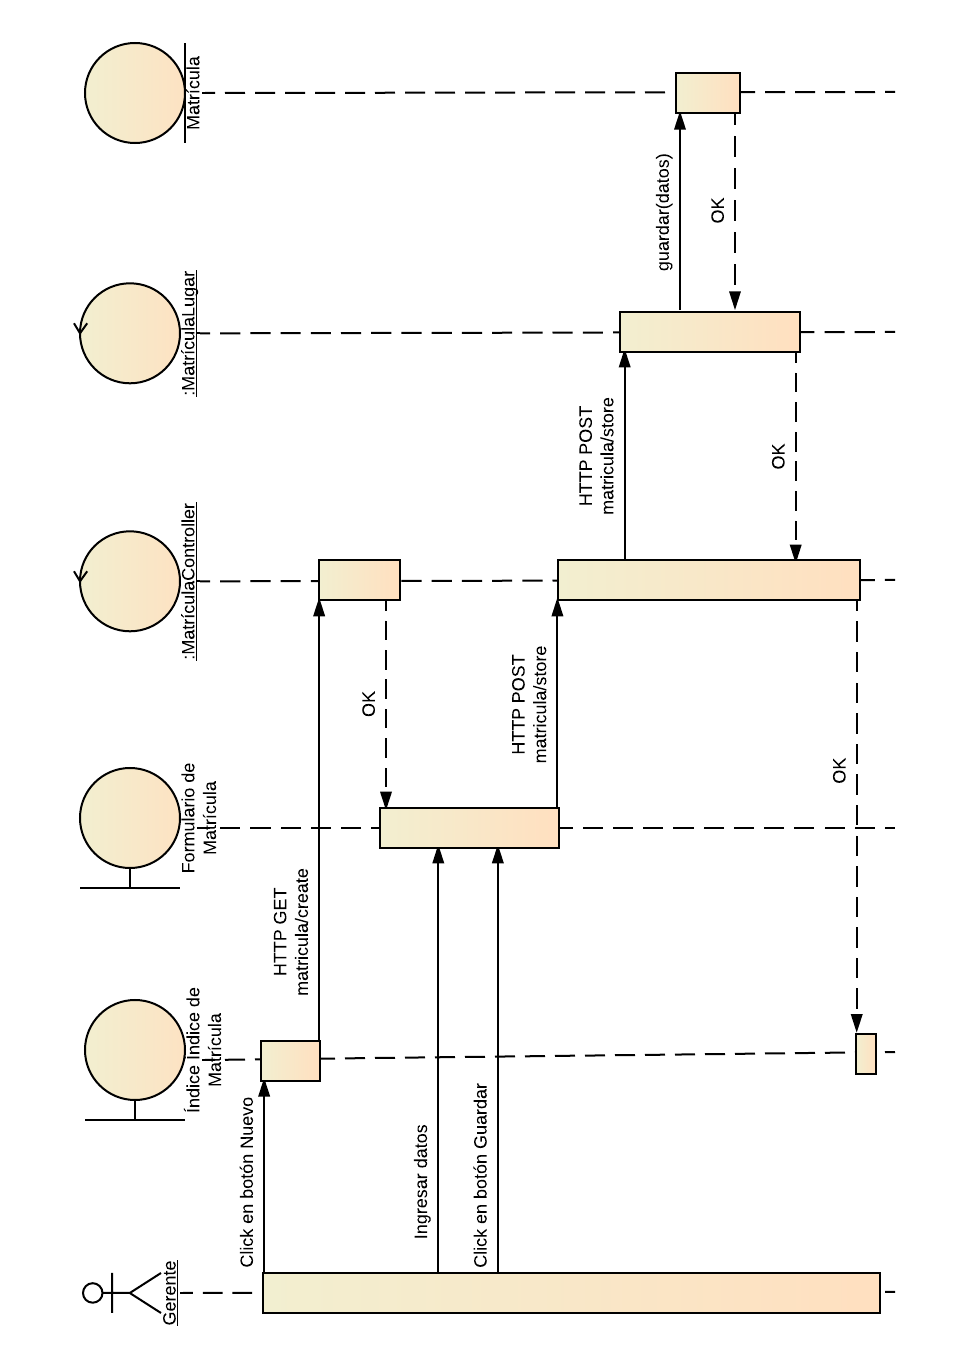
\includegraphics[width=1\textwidth]{chapter10/seq-matri-nu}
        \caption{Gestionar Matrícula - Diagrama de Secuencia (1) }
        \label{fig:seq-matri-nu}
    \end{figure}
    
    \begin{figure}[H]
        \centering
        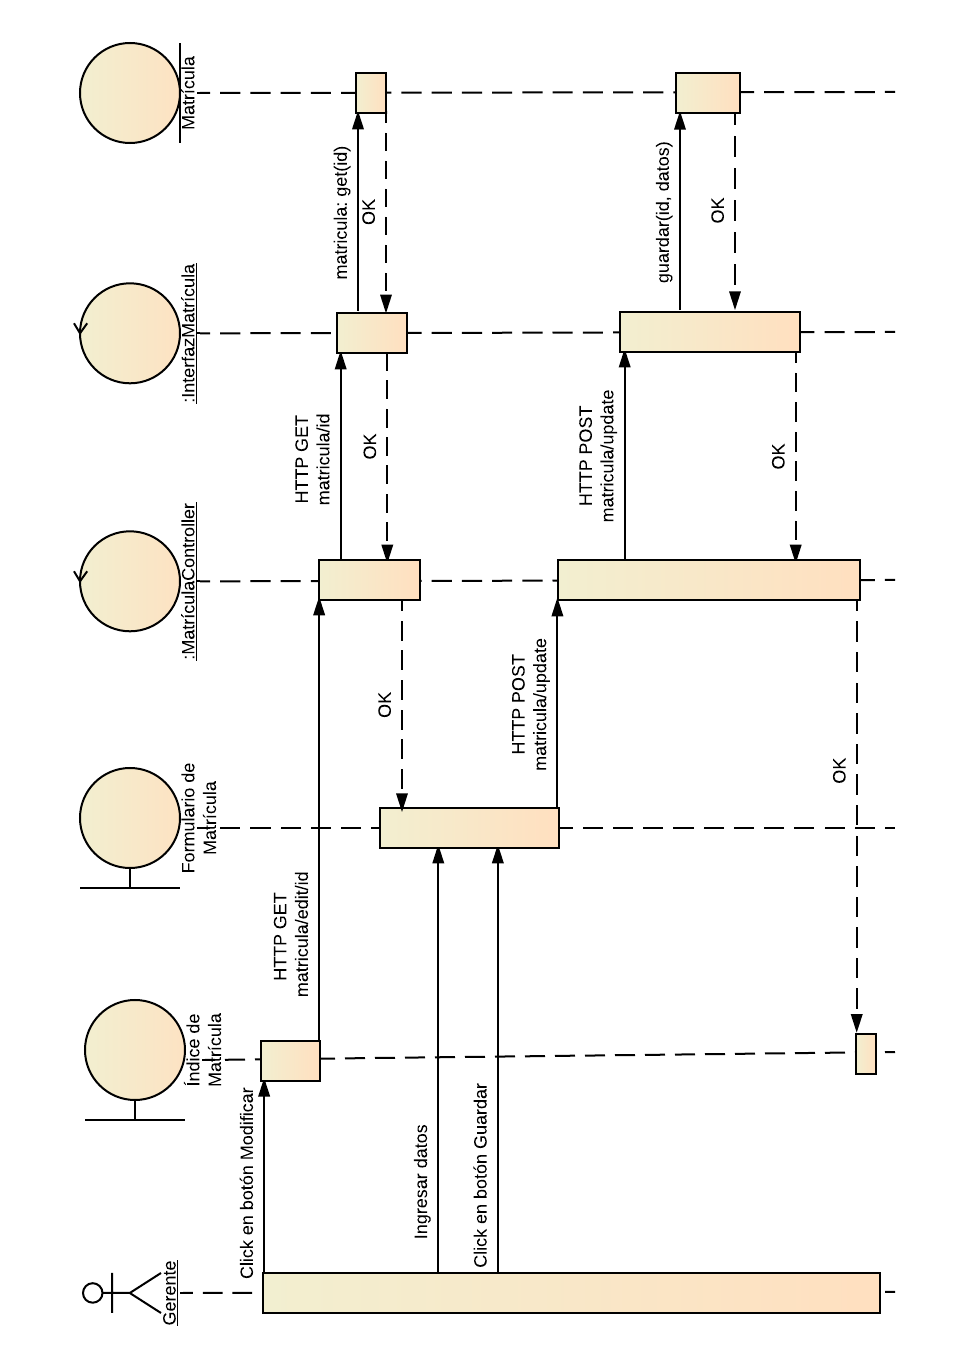
\includegraphics[width=1.1\textwidth]{chapter10/seq-matri-mod}
        \caption{Gestionar Matrícula - Diagrama de Secuencia (2) }
        \label{fig:seq-matri-mo}
    \end{figure}
    
    \begin{figure}[H]
        \centering
        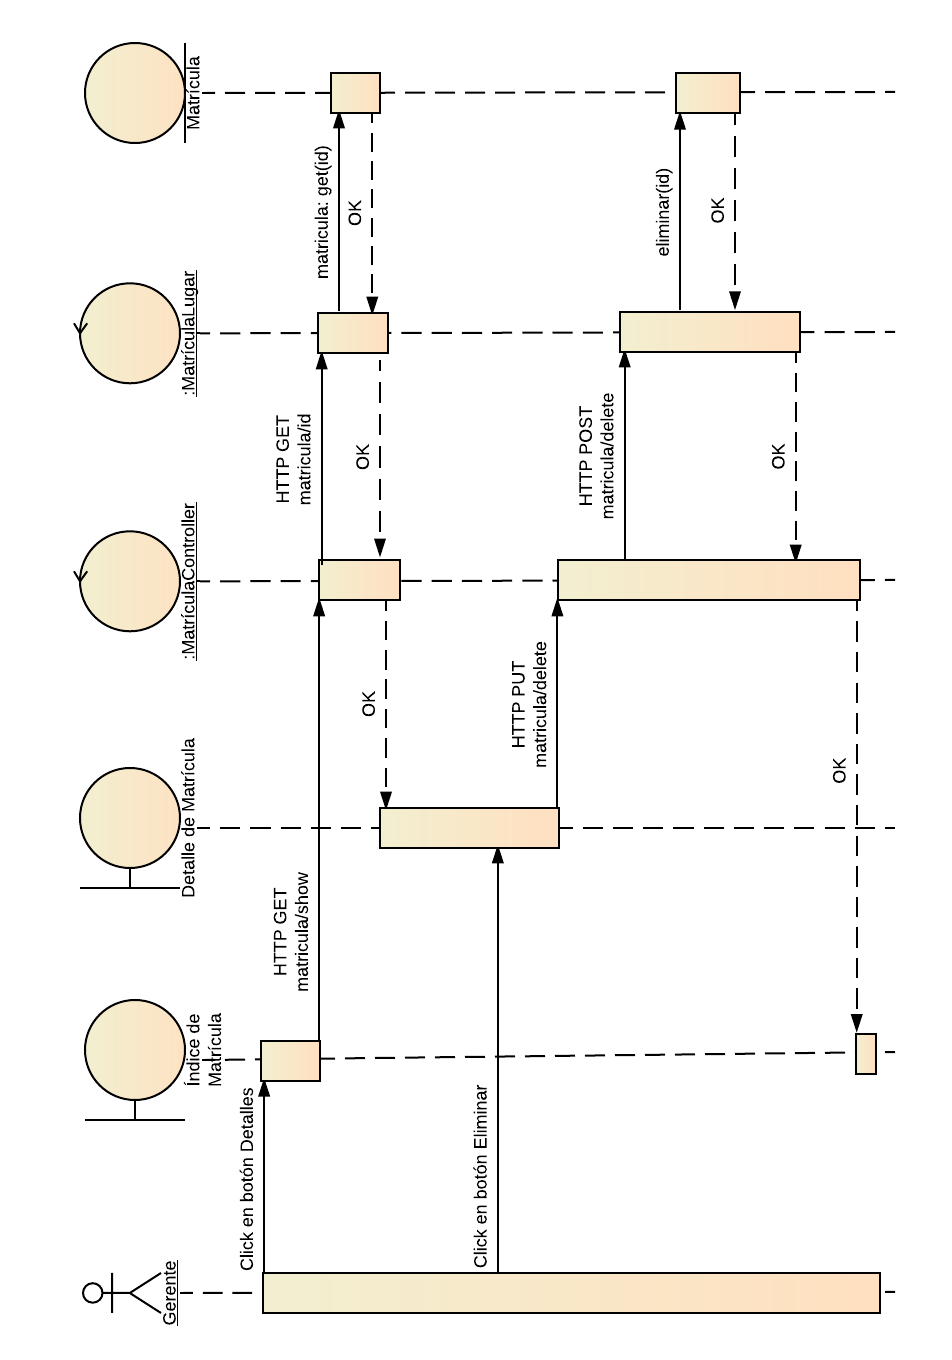
\includegraphics[width=1.1\textwidth]{chapter10/seq-matri-el}
        \caption{Gestionar Matrícula - Diagrama de Secuencia (3) }
        \label{fig:seq-matri-el}
    \end{figure}
\end{landscape}
    
\section{Gestionar Propietario}

\begin{table}[H]
    \begin{tabular}{@{} p{3cm} p{10cm} @{}} \toprule
    \textbf{Caso de Uso}    & Gestionar Propietario \\ \midrule
    Actor                   & Gerente \\ \cmidrule{1-2}
    Descripción             & El gerente gestiona un Propietario. La información de los propietarios la proporciona otra base de datos. No se permite hacer Altas, Bajas o Modificaciones de esta entidad, solo Lecturas. \\ \cmidrule{1-2}
    Propósito               & El gerente quiere gestionar un Propietario. \\ \cmidrule{1-2}
    Precondiciones          & El gerente inicia su navegador web. \\ 
                            & Existe el Propietario. \\ \cmidrule{1-2} 
    Postcondiciones         & \\ \cmidrule{1-2} 
                            & 1. El gerente visita la página de Propietarios. \\ 
    Curso Básico            & 2. El gerente hace click en el botón Detalles de un Propietario. \\
                            & 2.1 El sistema recupera los datos del Propietario para mostrar la pagina de detalles. \\ \cmidrule{1-2}
    Excepciones             & \\ \bottomrule
   \end{tabular}
        \caption{Gestionar Propietario - Caso de Uso (3)}
        \label{tab:tabcu-prop}
\end{table}

    \begin{figure}[H]
        \centering
        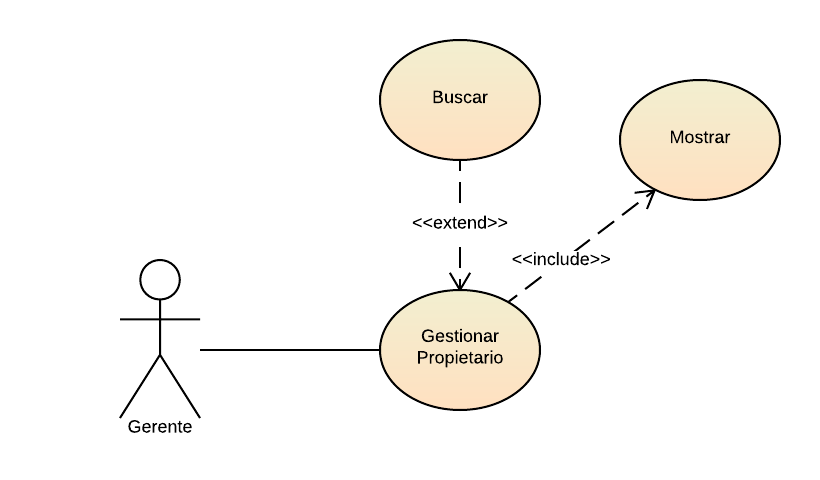
\includegraphics[width=.8\textwidth]{chapter10/uc-prop}
        \caption{Gestionar Propietario - Diagrama de Caso de Uso}
        \label{fig:uc-prop}
    \end{figure}
    
    % \begin{figure}[H]
    %     \centering
    %     \includegraphics[width=1\textwidth]{chapter10/camara-int}
    %     \caption{Gestionar Lugar - Interfaz Tentativa }
    %     \label{fig:lugar-int}
    % \end{figure}
    
    \begin{figure}[H]
        \centering
        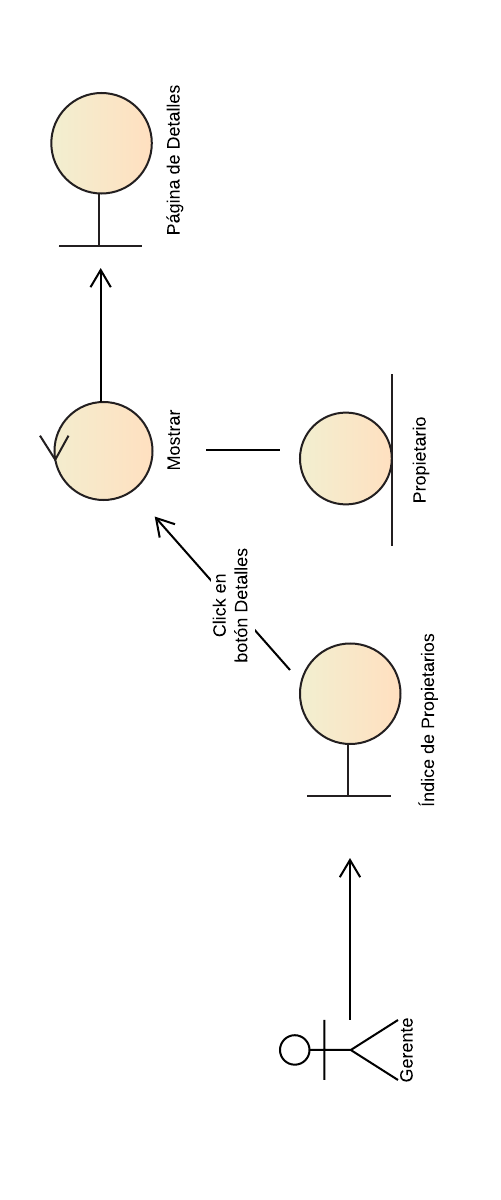
\includegraphics[width=.9\textwidth]{chapter10/rob-prop}
        \caption{Gestionar Propietario - Diagrama de Robustez}
        \label{fig:rob-prop}
    \end{figure}
    \begin{landscape}
        
    \begin{figure}[H]
        \centering
        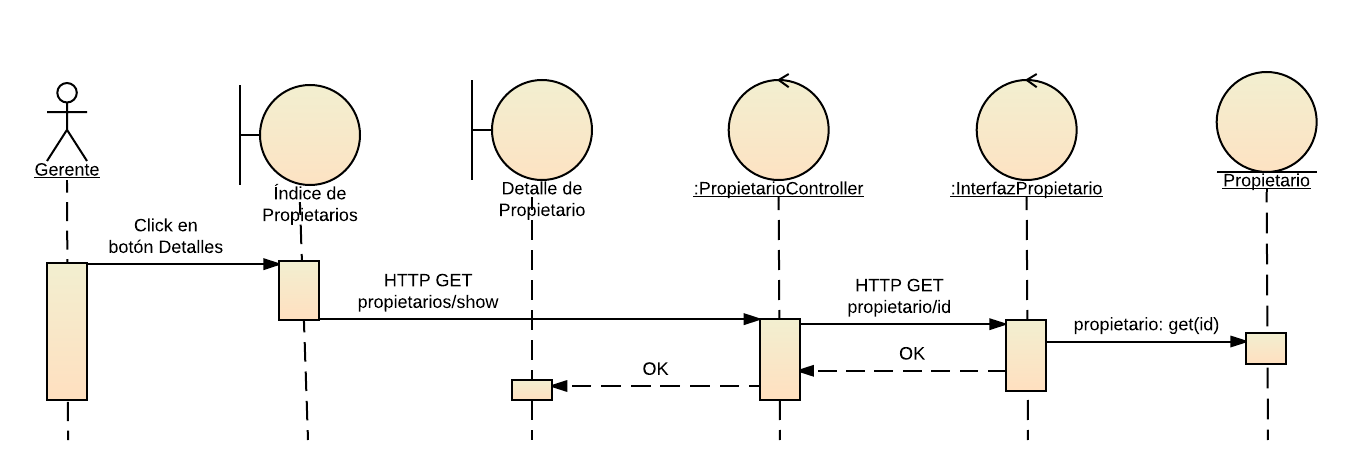
\includegraphics[width=1.2\textwidth]{chapter10/seq-prop}
        \caption{Gestionar Propietario - Diagrama de Secuencia (1) }
        \label{fig:seq-prop}
    \end{figure}
    \end{landscape}
    

\section{Gestionar Conexión a Cámara (Reconocer Matrícula)}

    \begin{longtable}{@{} p{3cm} p{10cm} @{}} \toprule
    \textbf{Caso de Uso}    & Reconocer Matrícula \\ \midrule
    Actor                   & Gerente \\ \cmidrule{1-2}
    Descripción             & El gerente inicia el servicio de reconocimiento para una cámara registrada. \\ \cmidrule{1-2}
    Propósito               & El gerente quiere que se realicen registros de coincidencias de matriculas a partir del vídeo de las cámaras de seguridad. \\ \cmidrule{1-2}
    Precondiciones          & El gerente inicia su navegador web. \\ 
                            & Existe la cámara. \\ \cmidrule{1-2} 
    Postcondiciones         & Existe un servicio de reconocimiento para la cámara (la conexión a la cámara esta establecida). \\ \cmidrule{1-2} 
                            & 1. El gerente visita la página de Cámaras. \\ 
                            & 2. El gerente hace click en el botón Conectar. \\
                            & 2.1 El sistema recupera la información de la cámara y la envía a un servicio recolector para asignar un servicio de recolección a la cámara seleccionada. \\
    Curso Básico            & 2.2. El sistema "recolecta" el flujo de vídeo y reenvía los cuadros del vídeo al servicio de reconocimiento. \\
                            & 2.3. El servicio de reconocimiento procesa los cuadros recibidos y envía  las matriculas reconocidas al servicio de almacenamiento. \\
                            & 2.4. El servicio de almacenamiento recupera la información correspondiente a la matricula reconocida y almacena la información asociada. \\ \cmidrule{1-2}
    Excepciones             & \\ \bottomrule
   \caption{Gestionar Propietario - Caso de Uso (3)} \label{tab:tabcu-matri}  \\
   \end{longtable}
       
    
    \begin{figure}[H]
        \centering
        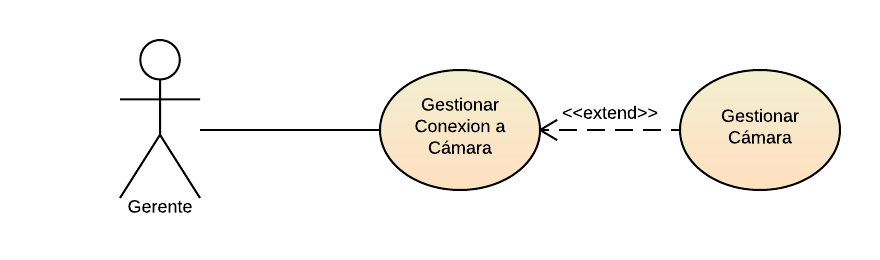
\includegraphics[width=.8\textwidth]{chapter10/uc-rec2}
        \caption{Gestionar Conexión a Cámara - Diagrama de Caso de Uso}
        \label{fig:uc-rec}
    \end{figure}
    \begin{landscape}
        
    \begin{figure}[H]
        \centering
        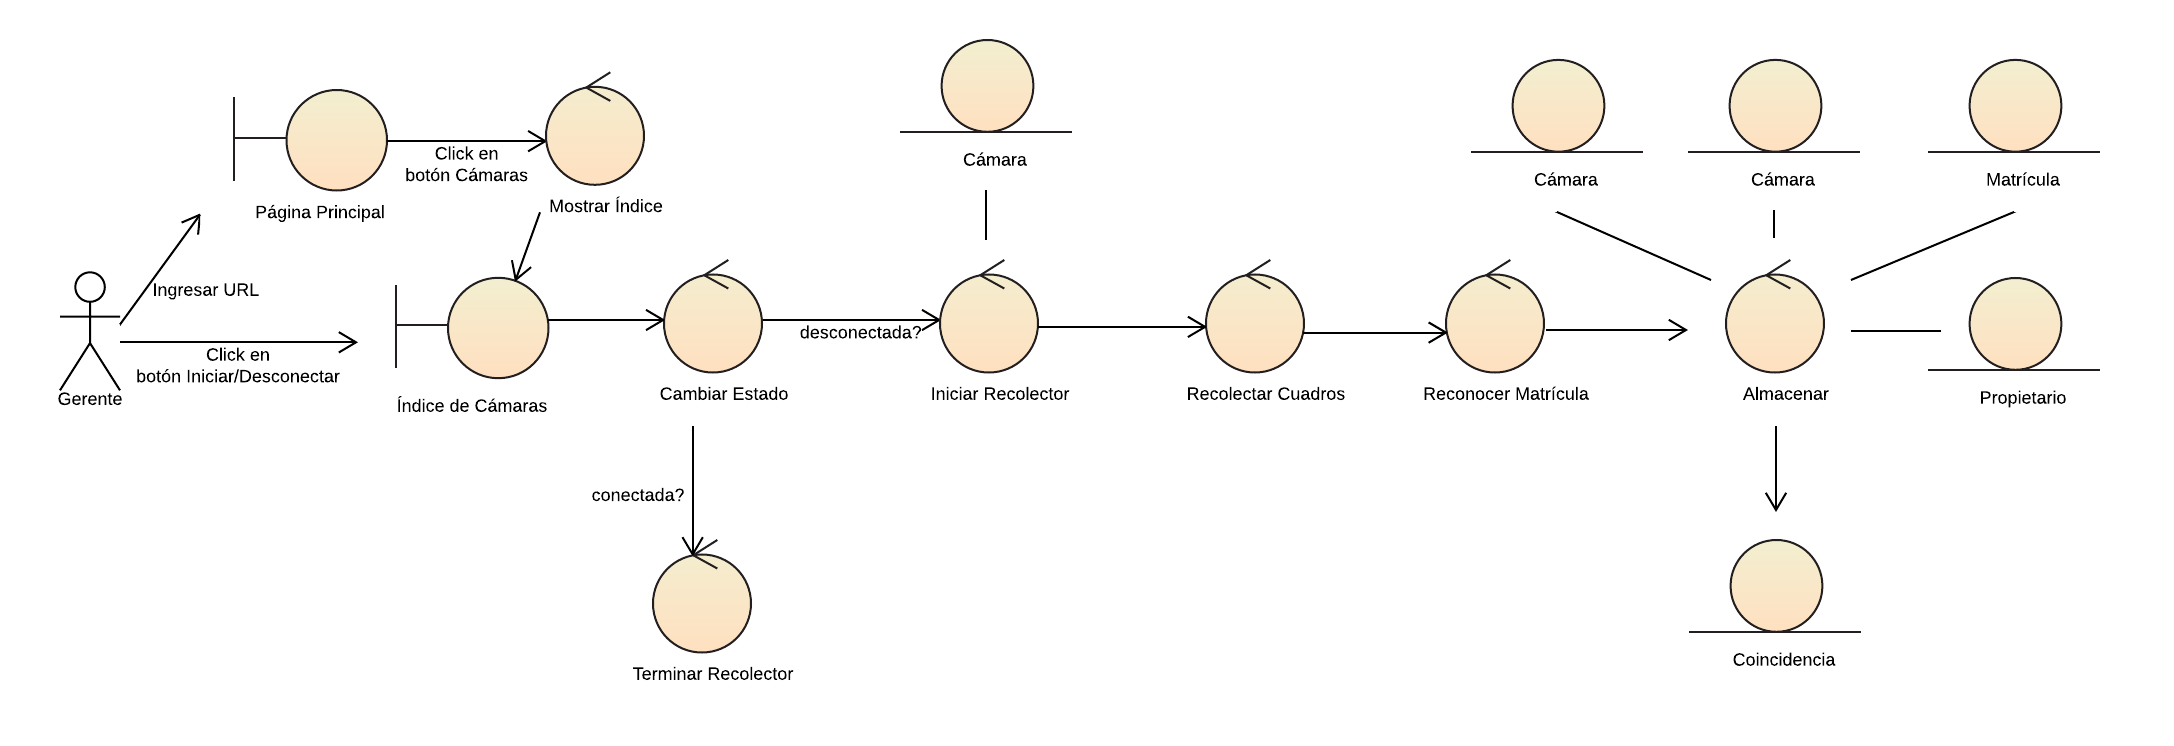
\includegraphics[width=1.4\textwidth]{chapter10/rob-rec}
        \caption{Gestionar Conexión a Cámara  - Diagrama de Robustez}
        \label{fig:rob-rec}
    \end{figure}
    
 \begin{figure}[H]
        \centering
        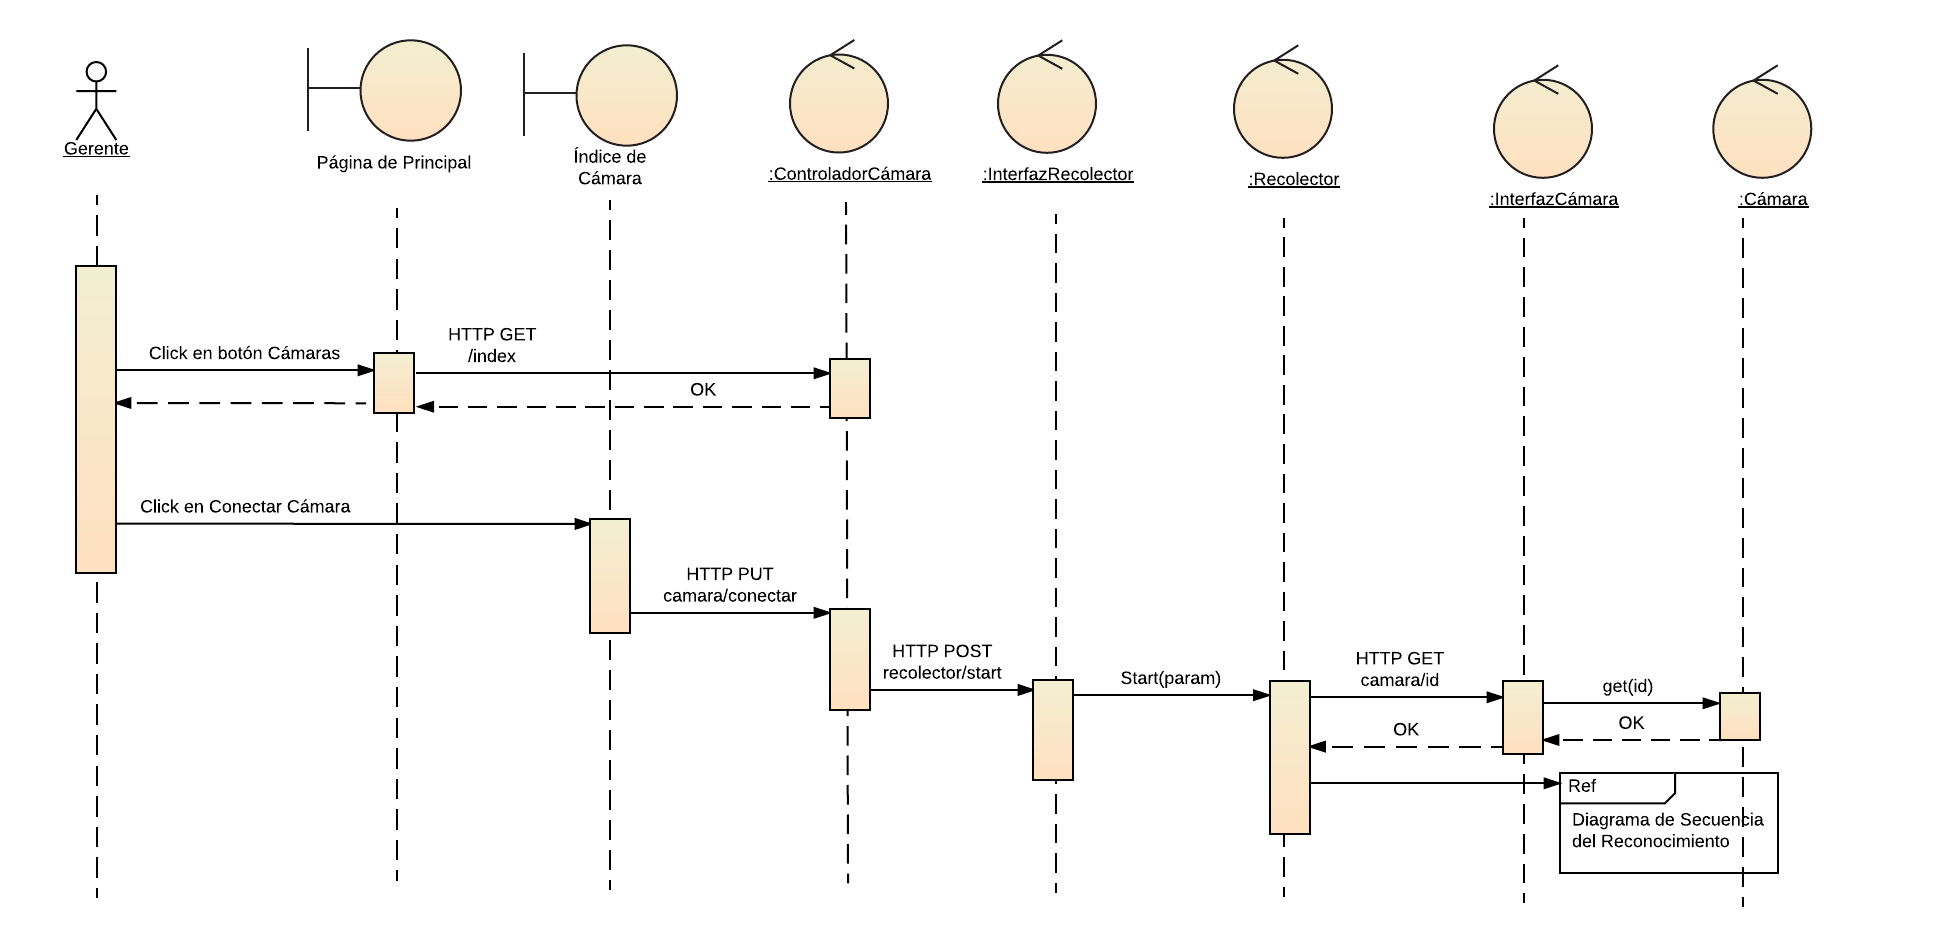
\includegraphics[width=1.2\textwidth]{chapter10/seq-recol}
        \caption{Gestionar Conexión a Cámara - Diagrama de Secuencia (1: Recolección)}
        \label{fig:seq-recol}
    \end{figure}
    
    \begin{figure}[H]
        \centering
        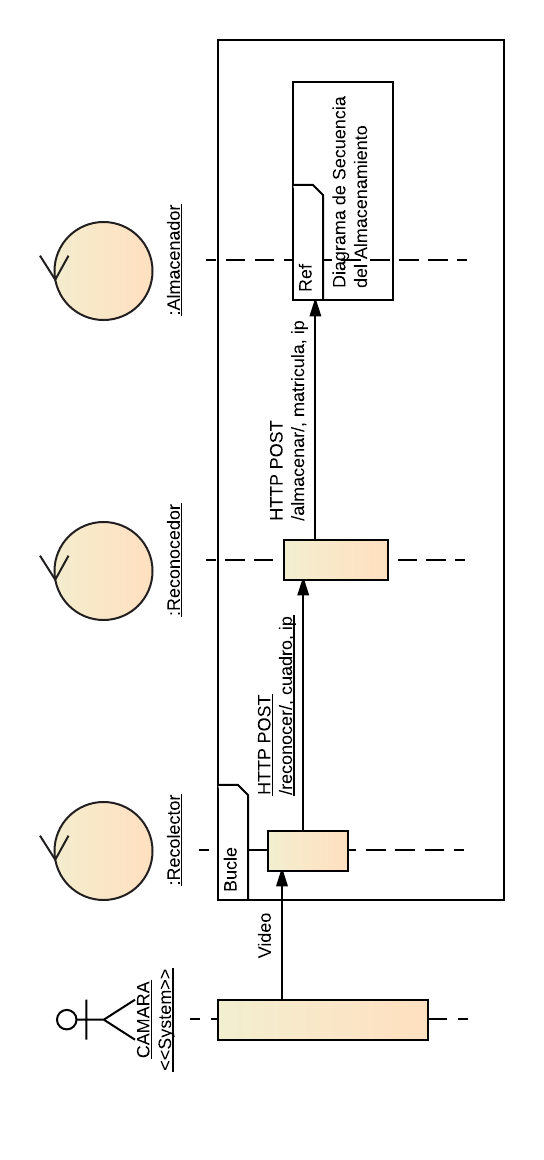
\includegraphics[width=1\textwidth]{chapter10/seq-rec}
        \caption{Gestionar Conexión a Cámara - Diagrama de Secuencia (1: Reconocimiento)  }
        \label{fig:seq-rec}
    \end{figure}
    
    \begin{figure}[H]
        \centering
        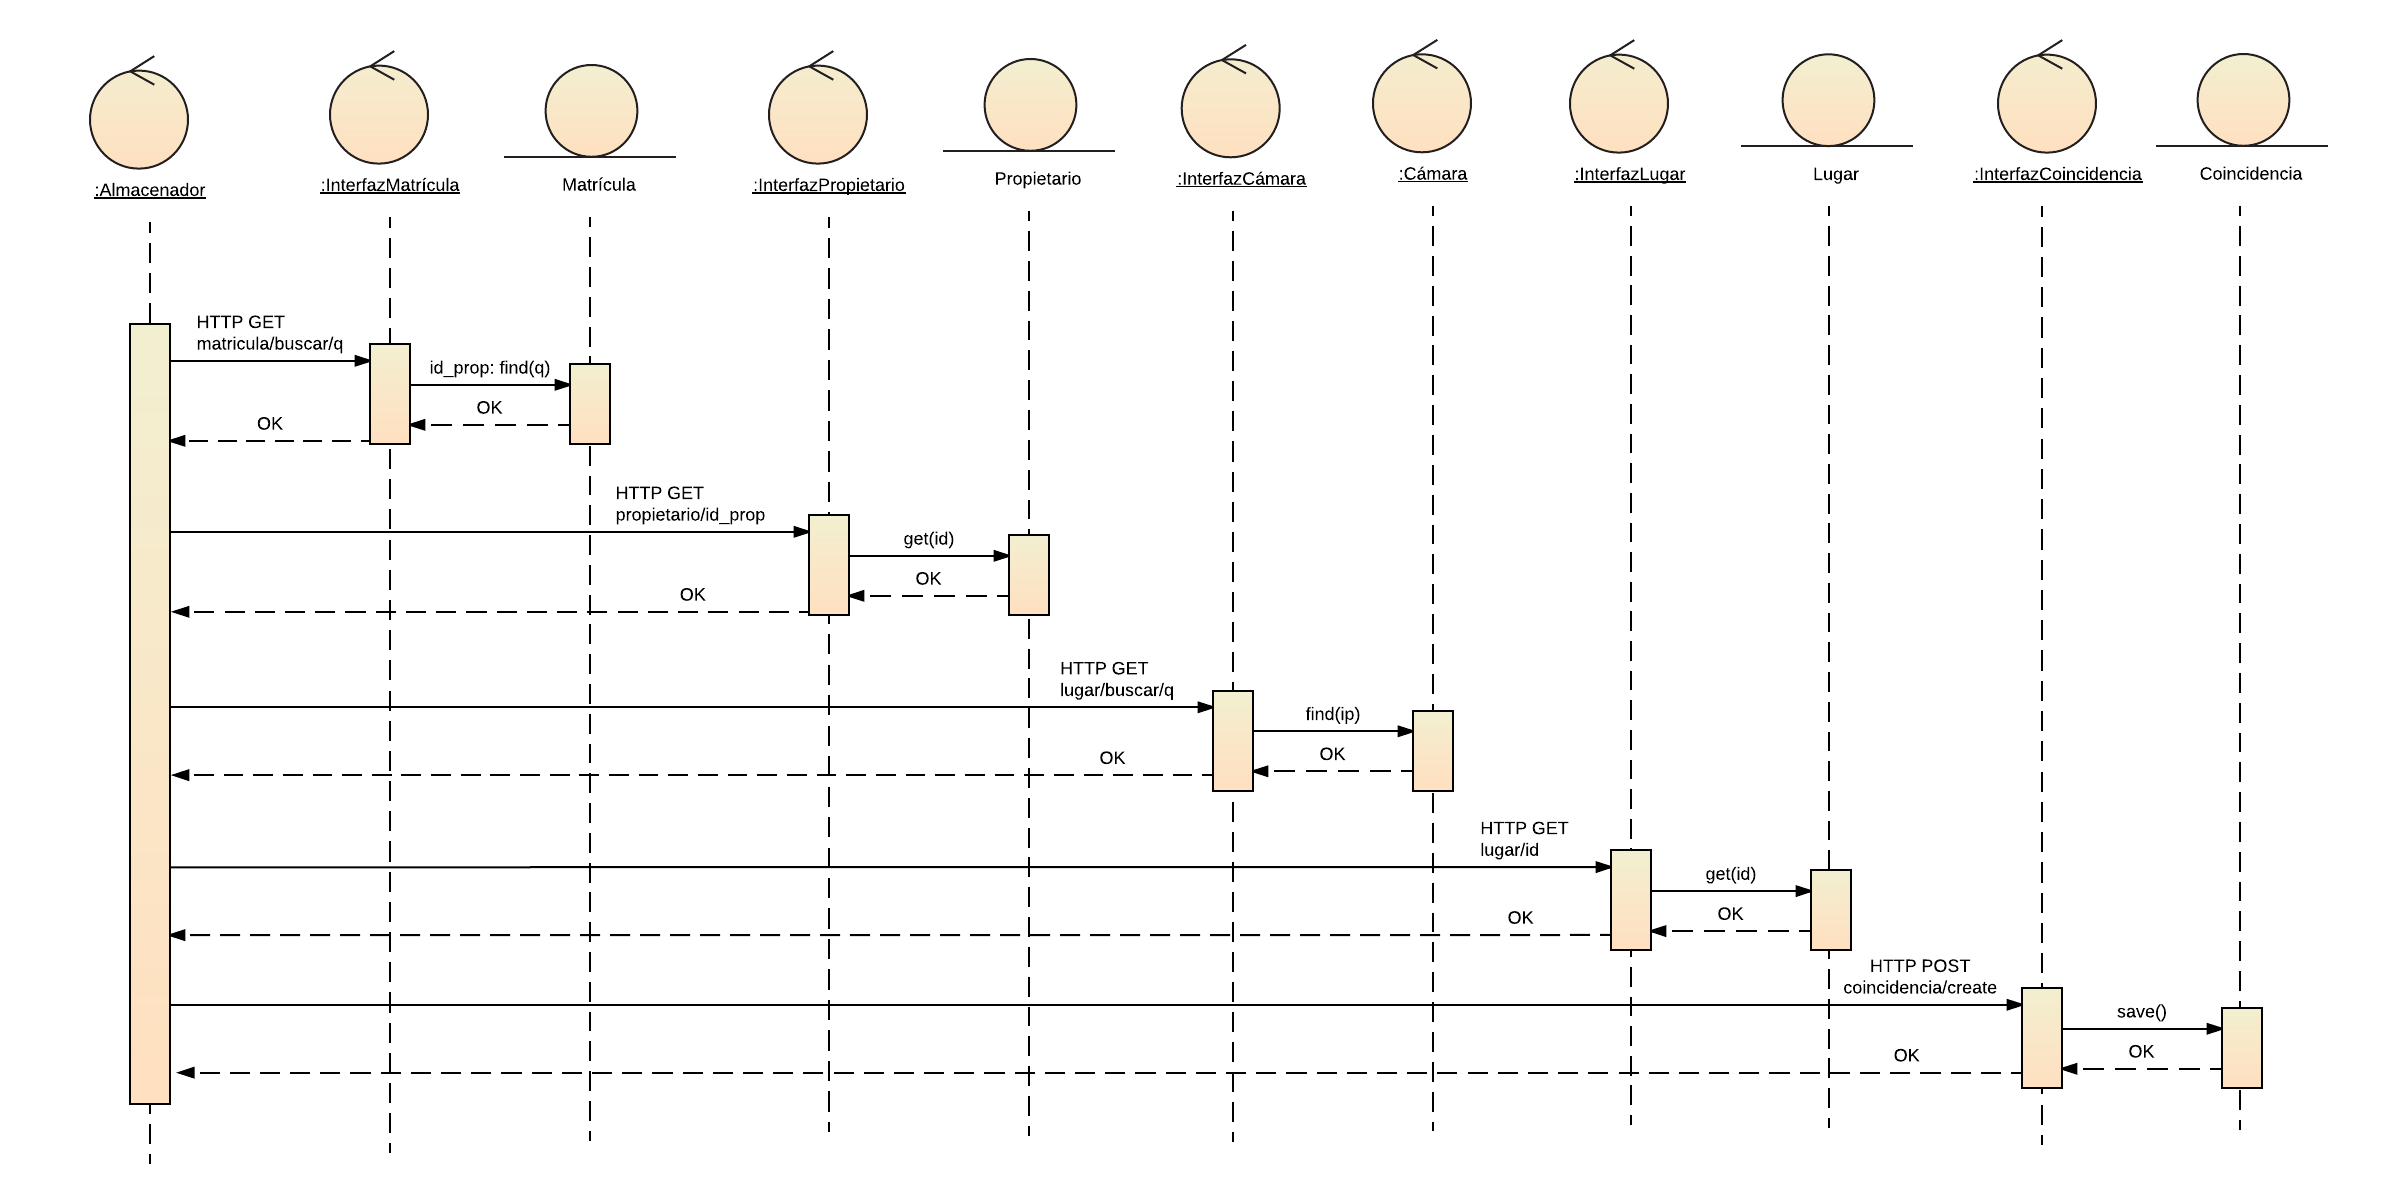
\includegraphics[width=1.4\textwidth]{chapter10/seq-alma}
        \caption{Gestionar Conexión a Cámara - Diagrama de Secuencia (3: Almacenamiento)  }
        \label{fig:seq-alma}
    \end{figure}
    \end{landscape}    
    
\section{Gestionar Coincidencia}

    \begin{longtable}{@{} p{3cm} p{10cm} @{}} \toprule
    \textbf{Caso de Uso}    & Reconocer Coincidencia \\ \midrule
    Actor                   & Gerente \\ \cmidrule{1-2}
    Descripción             & El gerente consulta la información correspondiente a una coincidencia (también llamada registro de matricula, registro de reconocimiento, o resultado de un reconocimiento), y la cual puede corresponder a un propietario que el sistema pueda encontrar o no. \\ \cmidrule{1-2}
    Propósito               & El gerente quiere consultar la información asociada a una coincidencia, esto puede ser imagen, propietario, fecha, lugar, o cámara. \\ \cmidrule{1-2}
    Precondiciones          & El gerente inicia su navegador web. \\ 
                            & Existe la coincidencia. \\ \cmidrule{1-2} 
    Postcondiciones         &  \\ \cmidrule{1-2} 
                            & 1. El gerente visita la página de Coincidencias. \\ 
    Curso Básico            & 2. El gerente hace click en el botón Detalles de una Coincidencia. \\
                            & 2.1 El sistema recupera la información de la coincidencia y muestra la pagina de Detalles. \\ \cmidrule{1-2}
    Excepciones             & \\ \bottomrule
   \caption{Gestionar Coincidencia - Caso de Uso} \label{tab:tabcu-coin}  \\
   \end{longtable}
    
    \begin{figure}[H]
        \centering
        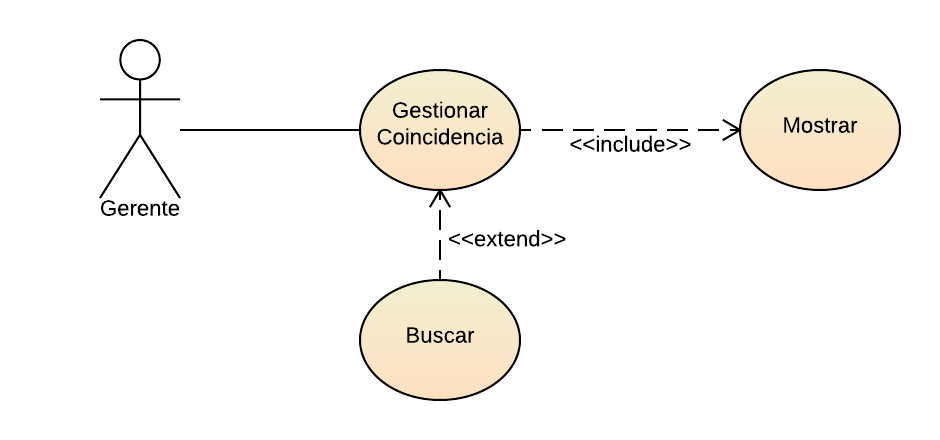
\includegraphics[width=0.85\textwidth]{chapter10/uc-coin}
        \caption{Gestionar Coincidencia - Diagrama de Caso de Uso}
        \label{fig:uc-coin}
    \end{figure}
    
    % \begin{figure}[H]
    %     \centering
    %     \includegraphics[width=1\textwidth]{chapter10/camara-int}
    %     \caption{Gestionar Lugar - Interfaz Tentativa }
    %     \label{fig:lugar-int}
    % \end{figure}
    \begin{landscape}
    \begin{figure}[H]
        \centering
        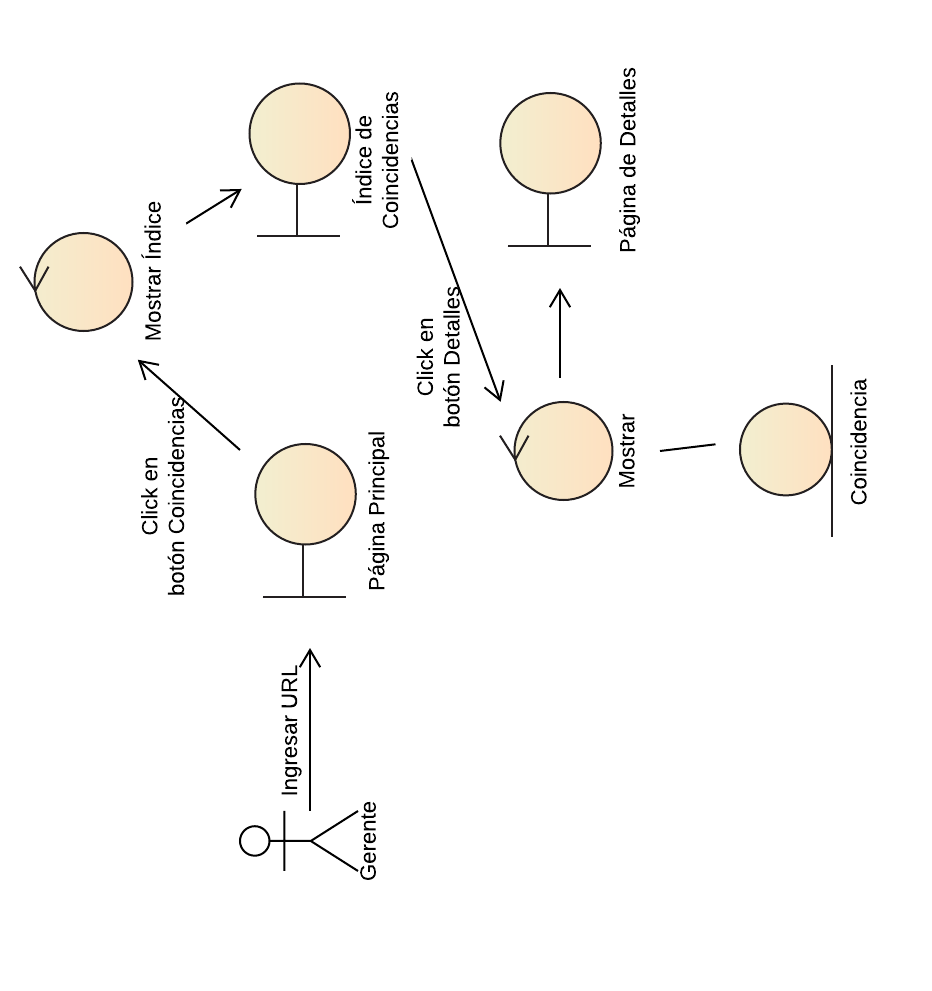
\includegraphics[width=1.2\textwidth]{chapter10/rob-coin}
        \caption{Gestionar Coincidencia - Diagrama de Robustez}
        \label{fig:rob-coin}
    \end{figure}
    
    \begin{figure}[H]
        \centering
        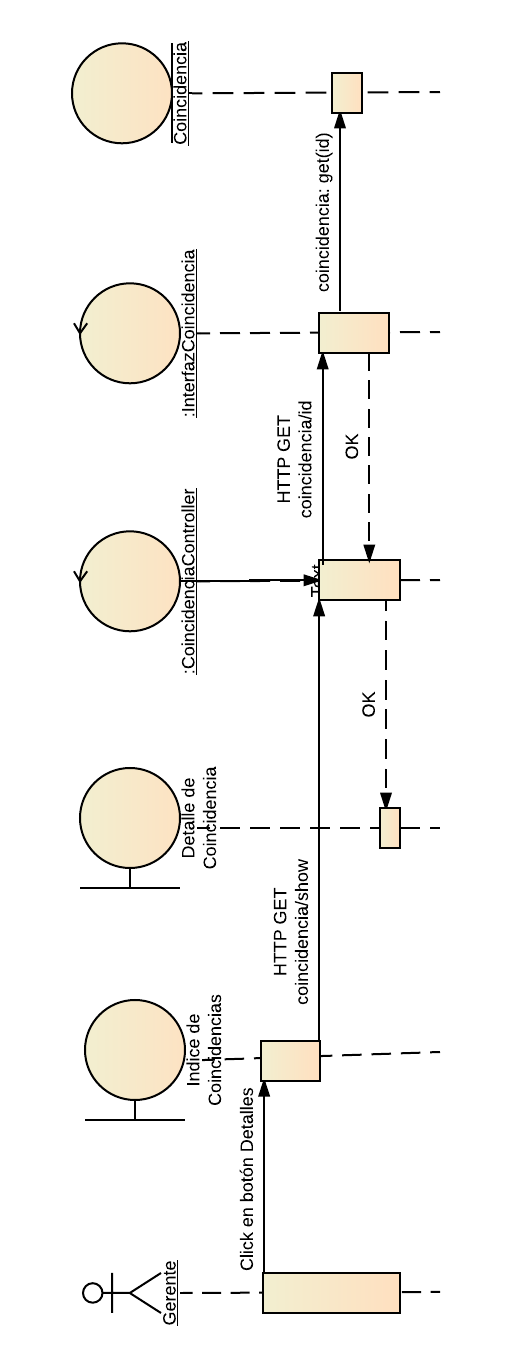
\includegraphics[width=1.1\textwidth]{chapter10/seq-coin}
        \caption{Gestionar Coincidencia - Diagrama de Secuencia }
        \label{fig:seq-coin}
    \end{figure}
    \end{landscape}
    
    
\section{Buscar}

\begin{figure}[H]
        \centering
        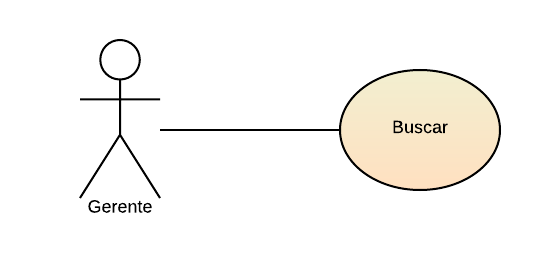
\includegraphics[width=0.7\textwidth]{chapter10/uc-buscar}
        \caption{Buscar - Diagrama de Robustez}
        \label{fig:uc-buscar}
    \end{figure}
    
 \begin{landscape}
    \begin{figure}[H]
        \centering
        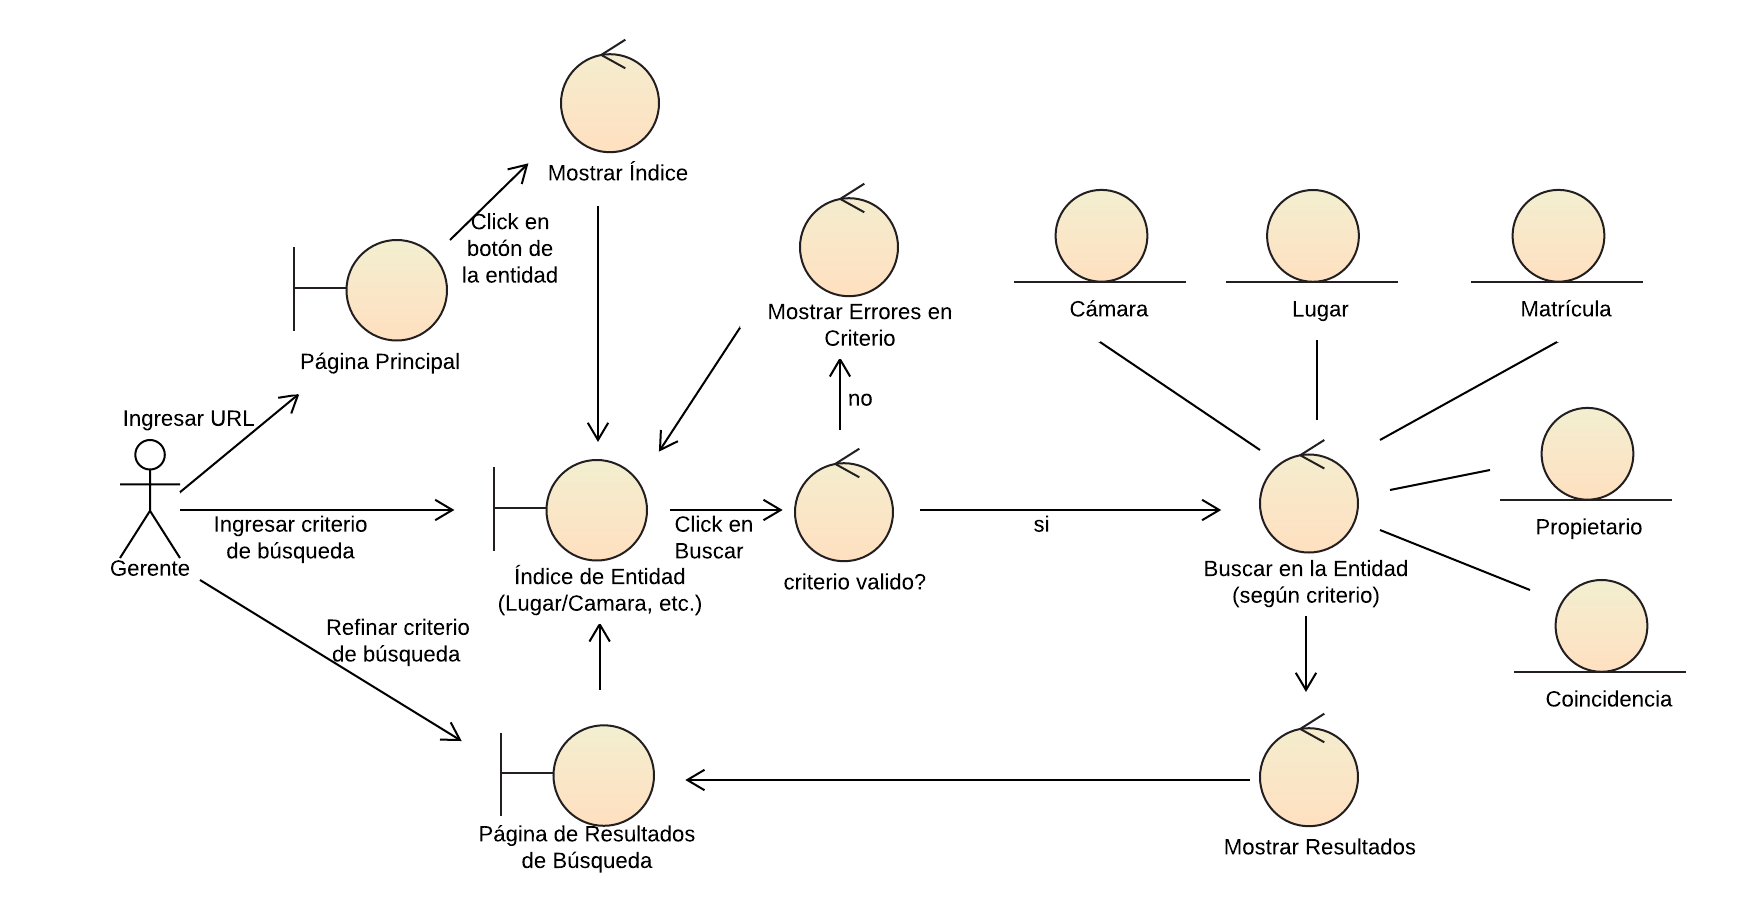
\includegraphics[width=1.2\textwidth]{chapter10/rob-buscar}
        \caption{Buscar - Diagrama de Robustez}
        \label{fig:rob-buscar}
    \end{figure}
    
    \begin{figure}[H]
        \centering
        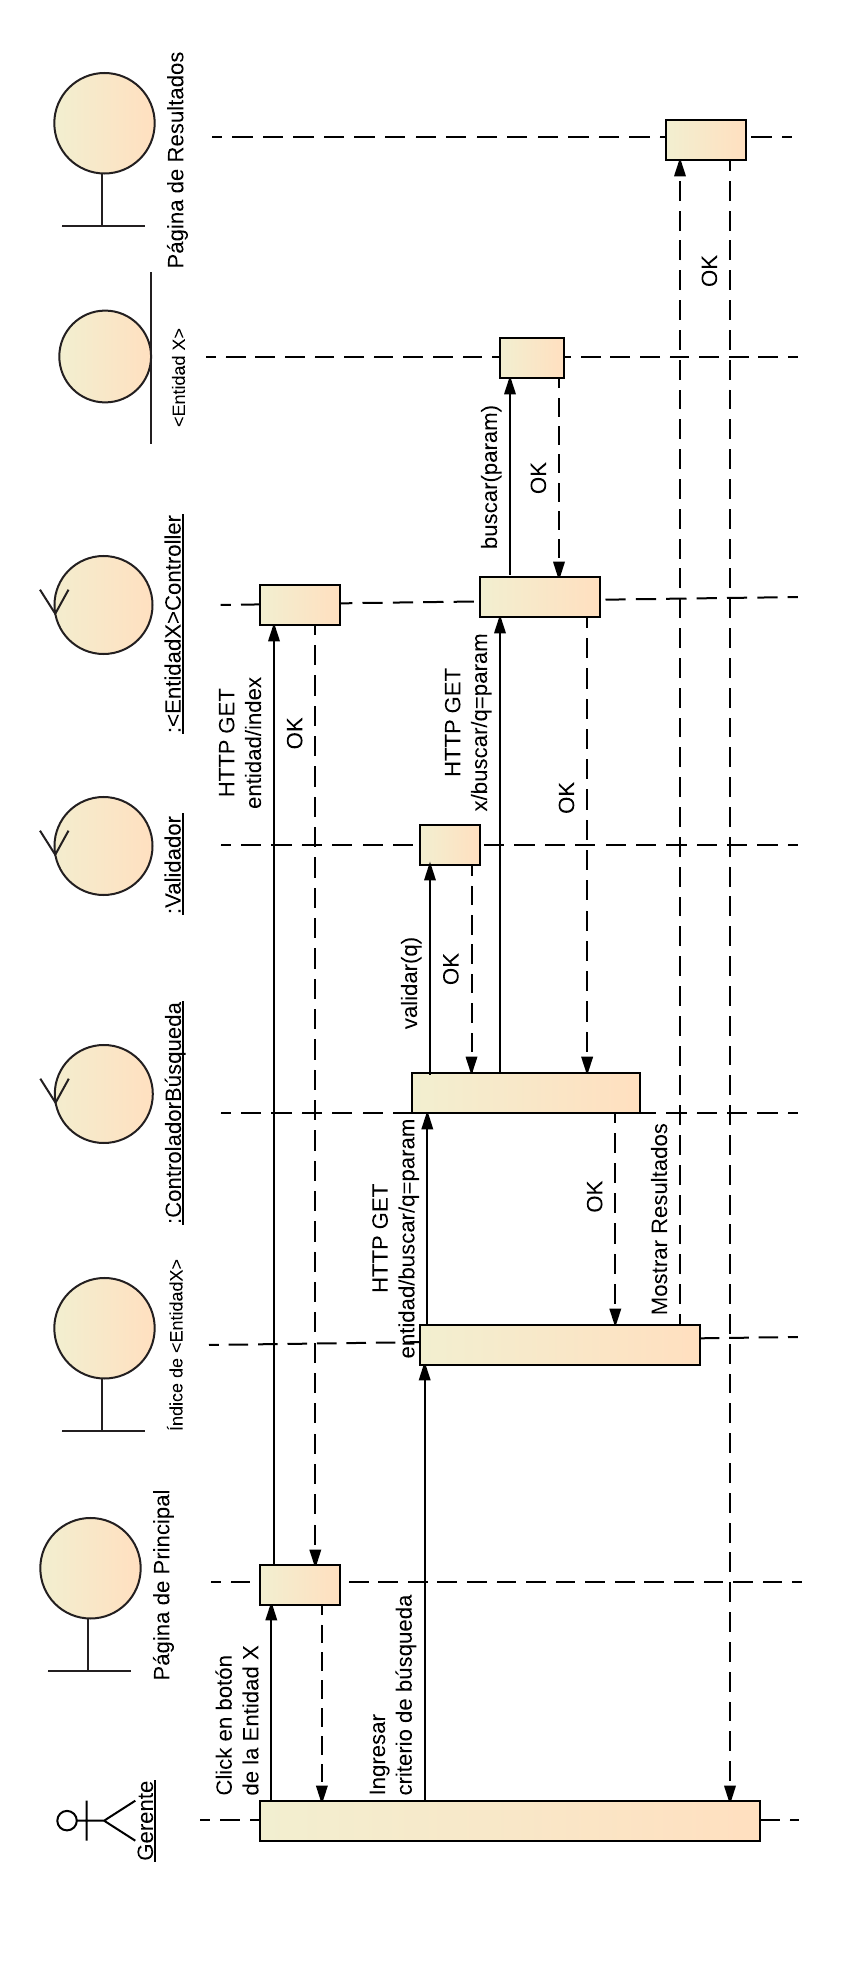
\includegraphics[width=1.3\textwidth]{chapter10/seq-buscar}
        \caption{Buscar - Diagrama de Secuencia }
        \label{fig:seq-buscar}
    \end{figure}
    \end{landscape}
    
\section{Gestionar Reporte}


\section{Diagrama de Despliegue}

\addtocontents{toc}{\protect\setlength{\cftsecnumwidth}{10mm}}